\chapter{Methods}
\label{methods}

This chapter describes the motivation behind the proposed \dettostoc{}, and outlines the algorithm in detail including the network architecture.

\section{Motivation}

%Combining deep learning with physics-based modeling has several positive benefits.  

Consider a physics simulator that correctly describes a dynamical system using laws of physics and mathematics. Since neural networks learn from experience, it is possible to learn the dynamics of this system and make accurate predictions given enough input and output samples.

%These networks are thus universal approximators, in their mapping of input vectors to output vectors, which is what makes them so useful for tasks in artificial intelligence. On the other hand, the sufficient number of hidden units of [26] is not guaranteed to be manageable computationally [27]. As is pointed out by Lin et al. in [27], the reason that a lot of neural network function approximations however indeed seem to work for a variety of tasks [25] is that the class of functions we are actually interested in is tiny, and essentially of low dimensionality, compared to the total collection of estimable functions.

General-purpose simulators like MuJoCo employ efficient dynamics models to make approximations but do not explicitly model uncertainty. MuJoCo is fast, however, in complex scenarios it is still time consuming to compute frictional contacts. In contrast, a forward pass in a neural network is fast, and a hybrid solution that combines deterministic simulators with learnable, stochastic neural networks allows for models that are efficient, expressive and generalizable.

%information from observed data, for example when there are unknown variables or parameters that cannot be measured, but we have observed data on how the system behaves.

The idea is to train a \cvae{} using real data. But instead of starting from random encoder and decoder weights, we will first align the decoder function $\fdecoder{}$ with the output of an existing general-purpose simulator $\fsimulator{}$. Instead of adding noise to real-world observations, we introduce noise during simulation by collecting a set of trajectories using a range of simulation engine parameters $\psi$.

Furthermore, real data comes with uncertainty. This uncertainty can be modelled with a generative model such as a \vae{}, and the slightly modified \cvae{} allows us to condition on current state. Moreover, we can use our prior knowledge in a bayesian manner to reason about sensible values that affect the environment.

Domain and dynamics randomization are powerful techniques to reduce the reality gap. However, as shown with experiments in \parencite{Chebotar2018}, using wide distribution for randomization can cause infeasible solutions that hinder policy learning, or sub-optimal and conservative policies.

%Prior knowledge (parameters to affect environment) pre training

\section{Proposed \dettostoc{} algorithm}
\label{det2stoc:algorithm}

Our approach specifies how existing general-purpose simulators could be used to make the learning of the stochastic function $g(\cdot)$ more data efficient. Finally the \cvae{} is trained on the \emph{real} data. We denote real observations $\trajreal$ and simulated observations $\trajsim$.

\todo[inline]{Make this prettier.}

\begin{enumerate}[label=\textit{Step \arabic*}]
    \item \label{det2stoc:step1} Choose relevant simulator parameter space $\vpsi$
    \item \label{det2stoc:step2} Initialize $\vpsi$ (randomly or with initial estimates)
    \item \label{det2stoc:step3} Sample from $\vpsi$ and train $\fdecoder{}$ to match output of $\fpsisimulator{}$ 
    \item \label{det2stoc:step4} Train \cvae{} using pre-trained $\fdecoder{}$ with real observations $\trajreal$, keeping the first layer of the decoder frozen
    % \item \label{det2stoc:step5} Compute $\vph_\mu$ and $\vph_\sigma$ for $\qphi \given{\vz}{\vns^{(real)}, \vs^{(real)}, \va^{(real)}}$.
    %\item \label{det2stoc:step6} \emph{Evaluate log likelihood $\mathcal{L} = p \given{\vns^{(real)}}{\vs^{(real)}, \va^{(real)}, \vz}, \vz \sim \N(\vph_{\mu}, \vph_{\sigma})$. If $\mathcal{L}$ improves, go to step 2,  replacing previous simulation parameters with $\vph_{\mu}, \vph_{\sigma}$ learned with variational inference in \subref{det2stoc:step4}}
    %^\item \label{det2stoc:step7} \emph{Train \cvae{} using real-world data.}

    \item \label{det2stoc:step5} Go to \ref{det2stoc:step3}, replacing previous simulation parameters $\vpsi$ with the posterior $\vph_{\mu}$, $\vph_{\sigma}$ learned with variational inference in \ref{det2stoc:step4}
\end{enumerate}


%\begin{wrapfigure}{r}{1.0\textwidth}
%\vspace{-2px}
\begin{algorithm}[H]
%  \LinesNumberedHidden
  \DontPrintSemicolon
  $\trajreal \leftarrow$ collect real trajectories \;
  $\vpsi_0 \leftarrow$ initialize sim parameters \;
  \For{i $\in \{0, ..., N\}$}{
    $\trajsim_{\vpsi_i} \leftarrow$ collect sim trajectories from $\fsimulator{}(\vpsi_{i})$ \;
    %$\fdecoder{} \xleftarrow{}$ PreTrain($\trajsim$, $\vpsi_i$) \;
    $\ptheta \leftarrow$ train \fdecoder{} on $\trajsim_{\vpsi_i}$\;% \ptheta \given{\vns}{\vpsi_i, \vs, \va}$ \;
    %$f^{\cvae{}} \xleftarrow{}$ Train($\trajreal, \fdecoder{}$) with \fdecoder{} frozen\;
    $\qphi \leftarrow$ train \cvae{} using frozen $\fdecoder{}$ on $\trajreal$ \;
    $\vph_{\mu, \sigma} \leftarrow$ compute posterior $\qphi$ given $\trajreal$\;% $\qphi \given{\vz}{\vs, \va, \vns} $\;%($\trajreal, f^{\cvae{}}$) \;
    $\vpsi_{i+1} \xleftarrow[]{} \vph_{\mu, \sigma}$ \;
    %update parameter distribution from posterior given $\trajreal$ \;
  } % end for N robot trials
  \caption{det2stoc}
  \label{alg:det2stoc}
\end{algorithm}
%\vspace{-10px}
%\end{wrapfigure}

In \ref{det2stoc:step1}, we choose a set of parameters $\vpsi$ that cannot be measured or that have uncertainty associated with them.

In \ref{det2stoc:step2} we decide on an initial distribution for these values, typically an uninformative distribution, for example a uniform distribution or a wide truncated normal distribution. 

In \ref{det2stoc:step3}, we run simulations parameterized by samples from $\vpsi$ and collect trajectories $\trajsim_{\vpsi}=\{\vs, \va, \vns\}^{1:N}$. The decoder network is trained separately on the simulated data $\trajsim_{\vec{\psi}}{}$ using a negative log likelihood loss function. However, during this pre-training phase, instead of sampling $\vz$ from the prior or posterior, the network is fed parameters $\vpsi$ used during simulation for that particular timestep $\fdecoder = f(\vpsi; \vth)$. The intention of this step is to train the decoder to capture how the physics parameters affect the system dynamics which will infer parameters $\vpsi_\mu$, $\vpsi_\sigma$ that closely ressemble those of real-world dynamics.

In \ref{det2stoc:step4}, the \cvae{} is trained to match $\fpsisimulator{}$, but the first layer of decoder weights is frozen. The purpose of this step is to train the encoder to produce a posterior that maximizes the log likelihood of the next state $\vns$, while ensuring that the decoder does not unlearn what it learned in \ref{det2stoc:step3}. The input to the encoder is state $\vs$, action $\va$ and next state $\vns$. %Including the next state ensures that there is enough information for the network to infer what parameter corresponds to which output.

In \ref{det2stoc:step5}, we update $\vpsi$ with the posterior $\vph_{\mu,\sigma}$ and go back to \ref{det2stoc:step3}.

This process can be repeated multiple times. The result of the \dettostoc{} algorithm is the trained decoder as well as the learned $\vph_{\mu, \sigma}$. Because of how the training procedure was set up, the network is now aligned with real world data.

%Since the \cvae{} includes the target $\vy$ in the posterior formulation, and we have trained the \cvae{} in a way that it is encouraged to represent the simulator parameters in latent space, we can perform system identification using variational inference and sampling from the posterior $q_{\vth} \given{\vz}{\vx,\vy}$. The idea is that if the \cvae{} has been trained on sufficiently many samples, it should be able to produce a posterior that in fact matches the parameter value that best predict the next state $\vns$.

\begin{figure}
\todo[inline]{This figure does not make much sense and is not pretty.}

\begin{subfigure}[t]{0.5\textwidth}
\centering
\begin{tikzpicture}[shorten >=1pt,->,draw=black!50, node distance=\layersep and \layersep, myarrow/.style={-Stealth}]
    \tikzstyle{every pin edge}=[<-,shorten <=1pt]
    \tikzstyle{neuron}=[rectangle,draw=black,fill=white!50,minimum height=30pt, minimum width=30pt, inner sep=10pt]
    %\tikzstyle{probabilistic neuron}=[draw=black,ultra thick,fill=white!50,minimum size=30pt,inner sep=0pt]
    \tikzstyle{input neuron}=[neuron];
    \tikzstyle{output neuron}=[neuron];
    \tikzstyle{hidden neuron}=[neuron];%, minimum height=30pt, minimum width=90pt];
    \tikzstyle{annot}=[text centered];

    \scriptsize
    % Draw the nodes
    \node[input neuron] (I-1) at (0,0) {$\vns$};
    \node[input neuron, right of=I-1] (I-2) {$\vs$};
    \node[input neuron, right of=I-2] (I-3) {$\va$};

    \node[input neuron, above of=I-1] (e) {$q_{\vth}\given{\vz}{\vns, \vs, \va}$};
        
    \node[input neuron, above of=e] (phi-1) {$\vph_{\mu,\sigma}(\vns, \vs, \va)$};

    %\node[input neuron, right of=e, anchor=west] (CI-1) {$\vs$};
    %\node[input neuron, right of=CI-1] (CI-2) {$\va$};
    
    \node[hidden neuron, above of=e, yshift=\layersep] (z) {$z \sim \mathcal{N}(\vph_{\mu}, \vph_{\sigma})$};
    \node[hidden neuron, right of=phi-1, anchor=west] (d) {$p_{\vph}\given{\vns}{\vz, \vs, \va}$};
        
    \node[output neuron, above of=d] (ns) {$\hat{\pmb{s}}_{t+1}$};

    % Connect every node
    \foreach \source in {1,...,3}
        \draw [myarrow] (I-\source) -- node[sloped] {} (e);
        
    % \foreach \source in {1,...,2}
        % \draw [myarrow] (CI-\source) -- node[sloped] {} (d);
        
    \foreach \dest in {1,...,1}
        \draw [myarrow] (e) -- node[sloped] {} (phi-\dest);
    
    \foreach \source in {1,...,1}
        \draw [myarrow] (phi-\source) -- node[sloped] {} (z);
    \draw [myarrow] (z) -- node[sloped] {} (d);
    
    \foreach \source in {2,...,3}
        \draw [myarrow] (I-\source) -- node[sloped] {} (d);

    \draw [myarrow] (d) -- node[sloped] {} (ns);
    %\draw[decorate,decoration={brace,mirror,amplitude=10pt},-,thick,black]
    %    ($(I-1)+(-1,0)$) -- ($(I-3)+(-1,0)$) node [black,midway,xshift=-1.0cm] {$s_t$};
        
    %\draw[decorate,decoration={brace,amplitude=10pt},-,thick,black]
    %    ($(O-1)+(1,0)$) -- ($(O-3)+(1,0)$) node [black,midway,xshift=1.0cm] {$s_{t+1}$};
    
\end{tikzpicture}
\end{subfigure}
\quad
\begin{subfigure}[t]{0.5\textwidth}

\centering
\begin{tikzpicture}[shorten >=1pt,->,draw=black!50, node distance=\layersep and \layersep, myarrow/.style={-Stealth}]
    \tikzstyle{every pin edge}=[<-,shorten <=1pt]
    \tikzstyle{neuron}=[rectangle,draw=black,fill=white!50,minimum size=30pt,inner sep=10pt]
    \tikzstyle{probabilistic neuron}=[draw=black,ultra thick,fill=white!50,minimum size=30pt,inner sep=0pt]
    \tikzstyle{input neuron}=[neuron];
    \tikzstyle{output neuron}=[neuron];
    \tikzstyle{hidden neuron}=[neuron, minimum height=30pt, minimum width=90pt];
    \tikzstyle{annot}=[text centered];

    \scriptsize
    % Draw the nodes
    \node[input neuron] (I-1) at (0,0) {$\vs$};
    \node[input neuron, right of=I-1, anchor=east] (I-2) {$\va$};
    \node[input neuron, right of=I-2] (I-3) {$\vz \sim \mathcal{N}(0, I)$};
        
    %\node[neuron, above of=I-1, yshift=\layersep] (phi) {$\vph_{\mu, \sigma}$};
    
    %\node[input neuron, right of=e, anchor=west] (CI-1) {$\vs$};
    %\node[input neuron, right of=CI-1] (CI-2) {$\va$};
    
    %\node[hidden neuron, above of=phi] (z) {$z \sim p_{\vph}\given{\vz}{\vns, \vs, \va}$};
    \node[hidden neuron, above of=I-1, xshift=\layersep] (d) {$p_{\vph}\given{\vns}{\vz, \vs, \va}$};
        
    \node[output neuron, above of=d] (ns) {$\hat{\vec{s}}_{t+1}$};

    % Connect every node
    
    %\draw [myarrow] (z) -- node[sloped] {} (d);
    
    \foreach \source in {1,...,3}
        \draw [myarrow] (I-\source) -- node[sloped] {} (d);

    \draw [myarrow] (d) -- node[sloped] {} (ns);
    %\draw[decorate,decoration={brace,mirror,amplitude=10pt},-,thick,black]
    %    ($(I-1)+(-1,0)$) -- ($(I-3)+(-1,0)$) node [black,midway,xshift=-1.0cm] {$s_t$};
        
    %\draw[decorate,decoration={brace,amplitude=10pt},-,thick,black]
    %    ($(O-1)+(1,0)$) -- ($(O-3)+(1,0)$) node [black,midway,xshift=1.0cm] {$s_{t+1}$};
        
\end{tikzpicture}
\end{subfigure}


\caption{(Left) A training-time \cvae{} network used for \dettostoc{}. The next state $\vns$ is only used as input to the encoder. The current state $\vs$ and action $\va$ are used as inputs to both encoder and decoder. (Right) A testing-time \cvae{} network. The current state $\vs$ and action $\va$ are used as inputs the decoder and we sample from a standard normal.}
\label{fig_gm_vae}
\end{figure}

\begin{figure}
\centering
\begin{tikzpicture}[shorten >=1pt,->,draw=black!50, node distance=\layersep and \layersep, myarrow/.style={-Stealth}]
    \tikzstyle{every pin edge}=[<-,shorten <=1pt]
    \tikzstyle{neuron}=[rectangle,draw=black,fill=white!50, minimum height=25pt, minimum width=50pt, inner sep=5pt]
    \tikzstyle{input neuron}=[neuron];
    \tikzstyle{output neuron}=[neuron];
    \tikzstyle{loss neuron}=[neuron, fill=pink];
    \tikzstyle{hidden neuron}=[neuron, minimum width=100pt];
    \tikzstyle{annot}=[text centered];

    \scriptsize
    % Draw the nodes
    \node[input neuron] (I-1) at (0,0) {$\vph_t^{sim}$};
    \node[input neuron, right of=I-1] (I-2) {$\vs$};
    \node[input neuron, right of=I-2] (I-3) {$\va$};
    
    \node[hidden neuron, above of=I-2] (d) {$p_{\vph}\given{\vns}{\vph_t^{sim}, \vs, \va}$};
        
    \node[hidden neuron, above of=d] (f) {$ \fdecoder (\vph_t^{sim}, \vs, \va)$};
    
    \node[loss neuron, above of=f] (loss) {$\Vert \fpsisimulator{} (\vs, \va) - \fdecoder{}(\vph_t^{sim}, \vs, \va) \Vert^2$};

    % Connect every node

    \foreach \source in {1,...,3}
        \draw [myarrow] (I-\source) -- node[sloped] {} (d);

    \draw [myarrow] (d) -- node[sloped] {} (f);
    
    \draw [myarrow] (f) -- node[sloped] {} (loss);
    %\draw[decorate,decoration={brace,mirror,amplitude=10pt},-,thick,black]
    %    ($(I-1)+(-1,0)$) -- ($(I-3)+(-1,0)$) node [black,midway,xshift=-1.0cm] {$s_t$};
        
    %\draw[decorate,decoration={brace,amplitude=10pt},-,thick,black]
    %    ($(O-1)+(1,0)$) -- ($(O-3)+(1,0)$) node [black,midway,xshift=1.0cm] {$s_{t+1}$};
        
\end{tikzpicture}
\caption{Pretraining decoder. Instead of sampling from the prior or posterior, the latent space is replaced by the simulator parameters to align the decoder with the simulator. Pink shows loss layers.}
\label{fig_pretrain_decoder}
\todo[inline]{This figure does not make much sense and is not pretty.}

\end{figure}

% \begin{figure}
% \centering
% \begin{tikzpicture}[shorten >=1pt,->,draw=black!50, node distance=\layersep and \layersep, myarrow/.style={-Stealth}]
%     \tikzstyle{every pin edge}=[<-,shorten <=1pt]
%     \tikzstyle{neuron}=[rectangle,draw=black,fill=white!50,minimum size=30pt,inner sep=0pt]
%     \tikzstyle{probabilistic neuron}=[draw=black,ultra thick,fill=white!50,minimum size=30pt,inner sep=0pt]
%     \tikzstyle{input neuron}=[neuron];
%     \tikzstyle{output neuron}=[neuron];
%     \tikzstyle{hidden neuron}=[neuron, minimum width=30pt, minimum height=90pt];
%     \tikzstyle{annot}=[text centered];

%     \scriptsize
%     % Draw the nodes
%     \node[input neuron] (I-1) at (0,0) {$\vns$};
%     \node[input neuron, below of=I-1] (I-2) {$\vs$};
%     \node[input neuron, below of=I-2] (I-3) {$\va$};

%     \node[hidden neuron, right of=I-2] (e) {$q$};
        
%     \node[neuron, right of=I-1, xshift=\layersep] (phi) {$\vph_{\mu, \sigma}$};
    
%     \node[input neuron, below of=phi] (CI-1) {$\vs$};
%     \node[input neuron, below of=CI-1] (CI-2) {$\va$};
    
%     \node[hidden neuron, right of=CI-1] (d) {$p$};
        
%     \node[output neuron, right of=d] (ns)  {$\vns$};

%     % Connect every node
%     \foreach \source in {1,...,3}
%         \draw [myarrow] (I-\source) -- node[sloped] {} (e);
        
%     \draw [myarrow] (e) -- node[sloped] {} (phi);
    
%     \draw [myarrow] (phi) -- node[sloped] {} (d);
    
%     \foreach \source in {1,...,2}
%         \draw [myarrow] (CI-\source) -- node[sloped] {} (d);

%     \draw [myarrow] (d) -- node[sloped] {} (ns);
%     %\draw[decorate,decoration={brace,mirror,amplitude=10pt},-,thick,black]
%     %    ($(I-1)+(-1,0)$) -- ($(I-3)+(-1,0)$) node [black,midway,xshift=-1.0cm] {$s_t$};
        
%     %\draw[decorate,decoration={brace,amplitude=10pt},-,thick,black]
%     %    ($(O-1)+(1,0)$) -- ($(O-3)+(1,0)$) node [black,midway,xshift=1.0cm] {$s_{t+1}$};
        
% \end{tikzpicture}
% \caption{A \cvae{} network. The thick border denotes a probabilistic neuron. The current state is fed to the decoder network along with the codings.}
% \label{fig_gm_vae}
% \end{figure}

\section{Conditioning architecture and transfer-aware training}

Motivating the architecture (eg skip connections etc). \todo{Experiment with Beta and prior and stddev on prior!}


\section{Implementation details}

Since the KL divergence term in the objective function penalizes priors that diverge from the standard normal distribution, the simulator parameters are scaled to have a mean of 0 and standard deviation of 1:

\begin{equation*}
    z = \frac{x - \mu}{\sigma}
\end{equation*}


Rather than trying to output the next state, the target $\vy$ is the delta between next and current state

\begin{equation*}
    \vy_{\Delta} = \vns - \vs
\end{equation*}


% \begin{figure}
% \centering
% \begin{tikzpicture}[shorten >=1pt,->,draw=black!50, node distance=\layersep and \layersep, myarrow/.style={-Stealth}]
%     \tikzstyle{every pin edge}=[<-,shorten <=1pt]
%     \tikzstyle{neuron}=[circle,draw=black,fill=white!50,minimum size=30pt,inner sep=0pt]
%     \tikzstyle{probabilistic neuron}=[circle,draw=black,ultra thick,fill=white!50,minimum size=30pt,inner sep=0pt]
%     \tikzstyle{input neuron}=[neuron];
%     \tikzstyle{output neuron}=[probabilistic neuron];
%     \tikzstyle{hidden neuron}=[neuron];
%     \tikzstyle{annot}=[text centered];

%     \scriptsize
%     % Draw the nodes
%     \foreach \name / \y in {1,...,2}
%         \node[input neuron] (I-\name) at (0,-0.5*\layersep-\y*\layersep) {$s_{t_{\name}}$};

%     \foreach \name / \y in {1,...,3}
%         \node[hidden neuron] at (\layersep,-\y*\layersep) (he-\name) {};
        
%     \node[neuron, right of=he-1] (p-1) {$\phi_{\mu}$};
%     \node[neuron, right of=he-2] (p-2) {$\phi_{ \Sigma}$};
%     \node[neuron, right of=he-3] (p-3) {$\epsilon$};
        
%     \foreach \name in {1,...,3}
%         \node[hidden neuron, right of=p-\name] (z-\name) {$z_{\name}$};
        
%     \foreach \name / \y in {1,...,3}
%         \node[hidden neuron, right of=z-\name] (hd-\name) {};

%     \foreach \name / \y in {1,...,2}
%         \node[output neuron, right of=hd-\name, yshift=-0.5*\layersep] (O-\name)  {$s_{{(t+1)}_{\name}}$};

%     % Connect every node
%     \foreach \source in {1,...,2}
%         \foreach \dest in {1,...,3}
%             \draw [myarrow] (I-\source) -- node[sloped] {} (he-\dest);
            
%     \foreach \source in {1,...,3}
%         \foreach \dest in {1,...,2}
%             \draw [myarrow] (he-\source) -- node[sloped] {} (p-\dest);
            
%     \foreach \source in {1,...,3}
%         \foreach \dest in {1,...,3}
%             \draw [myarrow] (p-\source) -- node[sloped] {} (z-\dest);
            
%     \foreach \source in {1,...,1}
%         \foreach \dest in {1,...,3}
%             \draw [myarrow] (z-\source) -- node[sloped] {} (hd-\dest);
            
%     \foreach \source in {1,...,2}
%         \foreach \dest in {1,...,3}
%             \draw [myarrow] (z-\source) -- node[sloped] {} (hd-\dest);

%     \foreach \source in {1,...,3}
%         \foreach \dest in {1,...,2}
%             \draw [myarrow] (hd-\source) -- node[sloped] {} (O-\dest);

%     %\draw[decorate,decoration={brace,mirror,amplitude=10pt},-,thick,black]
%     %    ($(I-1)+(-1,0)$) -- ($(I-3)+(-1,0)$) node [black,midway,xshift=-1.0cm] {$s_t$};
        
%     %\draw[decorate,decoration={brace,amplitude=10pt},-,thick,black]
%     %    ($(O-1)+(1,0)$) -- ($(O-3)+(1,0)$) node [black,midway,xshift=1.0cm] {$s_{t+1}$};
        
% \end{tikzpicture}
% \caption{A general representation of the network used for \dettostoc{}.}
% \label{fig_dettostoc}
% \end{figure}


\subsection{Tools}

The implementation was done in Python 3.5.2. Neural networks were built using TensorFlow \parencite{tensorflow2015-whitepaper}. 
All experiments were conducted on a machine with a Intel Core i7-8700 CPU, NVIDIA GeForce 1080Ti and 16GB of RAM.

\subsection{Network and training parameters}
Both the encoder and decoder networks consist of a 3-layer network with 64 units using ReLU activations and layer normalization \parencite{Ba2016}. The number of latent variables is equal to the number of variable parameters used when collecting the training data from simulation. The output from the encoder and decoder networks are multivariate normal distributions with diagonal covariance matrices.

%\subsubsection*{Latent variable collapse}
A common problem during training of a \vae{} is latent variable collapse. When this phenomenon occurs, the \vae{} learns a good generative model of the data but does not learn good representations of the individual data points. Specifically, when maximizing the lower bound of the log marginal likelihood, the posterior ''collapses'' at inference, when the posterior is set equal to the prior, essentially when the posterior is independent of the data. We combat this problem with skip-connections from the posterior to the decoder, essentially enforcing a stronger connection between the latent variables and the likelihood function \parencite{Dieng2018}.

Since the \cvae{} has the target $\vy$ in its posterior formulation, it is prone to overfitting unlike a regular \vae{} which tends to be regularized by the KL divergence term in the ELBO. The authors of \parencite{Sohn2015} suggest adding dropout to the encoder to combat this problem. A dropout rate of $0.5$ is used on the input layer to the encoder and helped avoiding extremely peaked latent encodings.

A learning rate of $1e^{-4}$ with a cosine decay is used to minimize the loss function using Adam \parencite{kingma2014adam}. We also employed early stopping for all parts of the training.

\subsection{Parameter space}

An important aspect of the method when using multiple parameters is to realize that the number of required samples increases exponentially with the number of parameters. It is crucial that the whole parameter space is covered for \dettostoc{} to be able to generalize to unseen data. Figure \ref{fig_parameter_space_3d} shows the parameter space in 3d for the Windy Slope scenario with friction, center of mass and wind.

\begin{figure}
\begin{center}
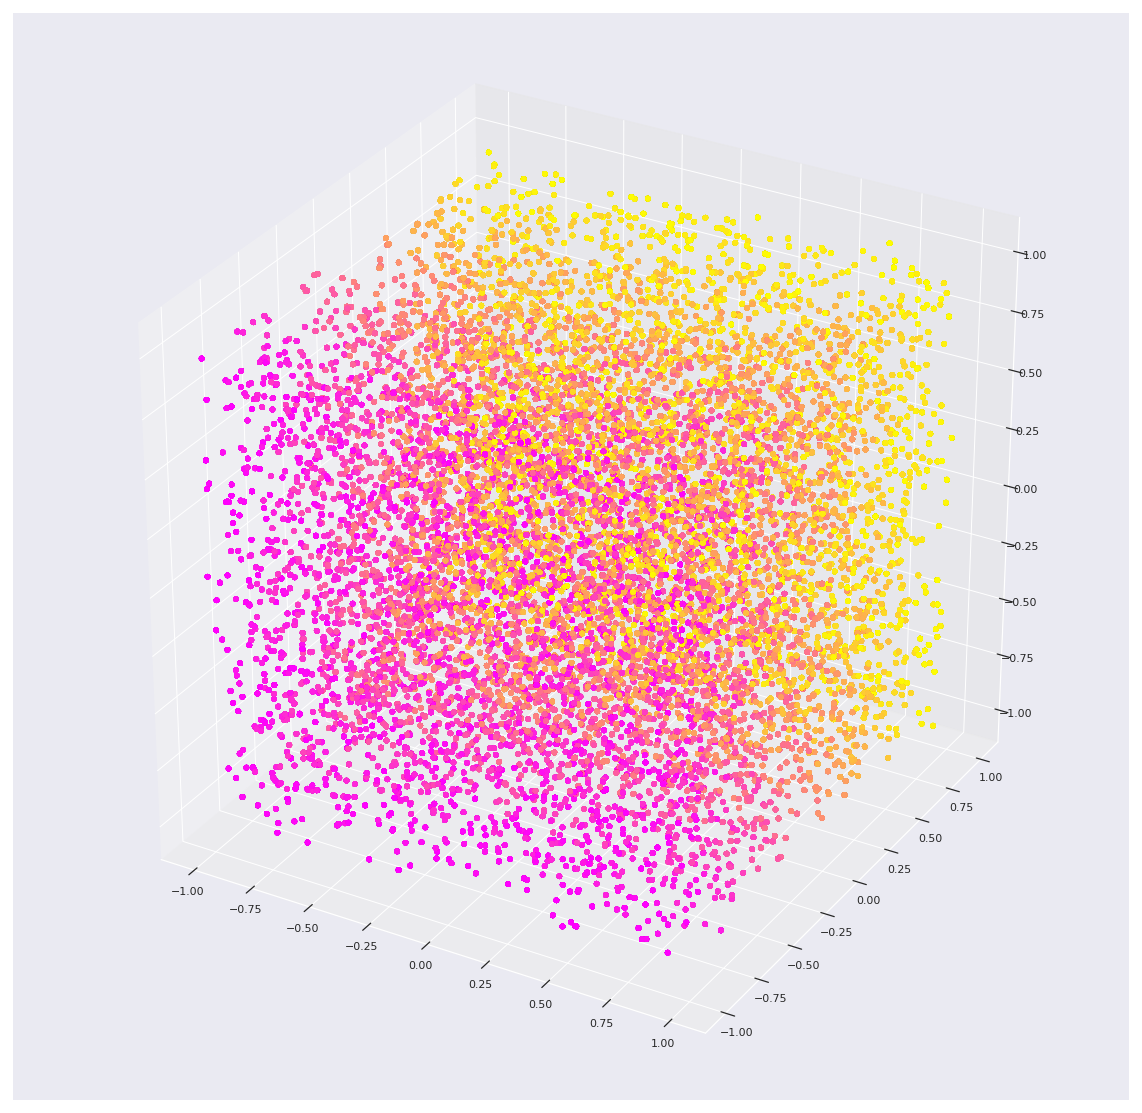
\includegraphics[width=0.8\textwidth]{img/parameter_space_3d}
\caption{A well covered parameter space in 3d.}
\label{fig_parameter_space_3d}
\end{center}
\todo[inline]{Not sure if this makes sense or is needed..}
\end{figure}

\chapter{Experimental results}
\label{experiments}

This chapter introduces in greater detail the data and results for the thesis project. We perform three experiments. The first is an analytic experiment, constructed as a proof of concept to confirm the basic premise that the \cvae{} can be used to predict conditional probabilities. In the following experiments we evaluate the \dettostoc{} algorithm in two different scenarios using MuJoCo.

Some questions we want to answer: How does \dettostoc{} compare against a baseline that has only trained on \emph{real} data? How many iterations of \dettostoc{} are required for \fdecoder{} to match \fsimulator{} with sufficient accuracy?


\section{Analytic experiment}
\label{exp:analytic}
As an initial experiment we use data with known distributions that can easily be analyzed. We define a joint distribution $p(s,a,s')$ and then attempt to learn the conditional distribution $p\given{s'}{s,a}$. If the distribution is a multivariate Gaussian, then the conditional distribution is also Gaussian and we can find analytic expressions for its mean and covariance. In the general case, if $\vec{Z}$ is a multivariate Gaussian variable of dimension $l+m$, we can partition $\vec{Z}$ into two multivariate variables $\vec{X}$ and $\vec{Y}$

\begin{equation}
\vec{Z} = 
\begin{bmatrix}
\vec{X} \\
\vec{Y}
\end{bmatrix}
\quad
\text{with sizes:} 
\begin{bmatrix}
l \\
m
\end{bmatrix}
\end{equation}
We then find their mean and covariance
\begin{equation}
\mu_{Z} = 
\begin{bmatrix}
\mu_{X} \\
\mu_{Y}
\end{bmatrix}
\quad
\text{with sizes:} 
\begin{bmatrix}
l \\
m
\end{bmatrix}
\end{equation}

\begin{equation}
\Sigma_{Z} = 
\begin{bmatrix}
\Sigma_{XX} & \Sigma_{XY} \\
\Sigma_{YX} & \Sigma_{YY}
\end{bmatrix}
\quad
\text{with sizes:} 
\begin{bmatrix}
l\times l & l \times m\\
m \times l & m \times m
\end{bmatrix}
\end{equation}
\\
The conditional distribution $p\given{\mathbf{X}}{\mathbf{Y}=\mathbf{y}}$ is then found by $\mathcal{N} (\mu_{\given{X}{Y}}, \Sigma_{\given{X}{Y}})$ where
\begin{align}
%\E[X \vert Y = y]
\mu_{\given{X}{Y}} &= \mu_{X} + \Sigma_{XY}\Sigma_{YY}^{-1}(y - \mu_{Y})
\label{eq_cond_mean}
\\
%Cov[X \vert Y = y]
\Sigma_{\given{X}{Y}} &= \Sigma_{XX} - \Sigma_{XY}\Sigma_{YY}^{-1}\Sigma_{YX}
\label{eq_cond_var}
\end{align}

The question is now is to see if it is possible to learn $\mu_{\given{X}{Y}}$ and $\Sigma_{\given{X}{Y}}$ using a \cvae{}.

\begin{figure}
\begin{center}
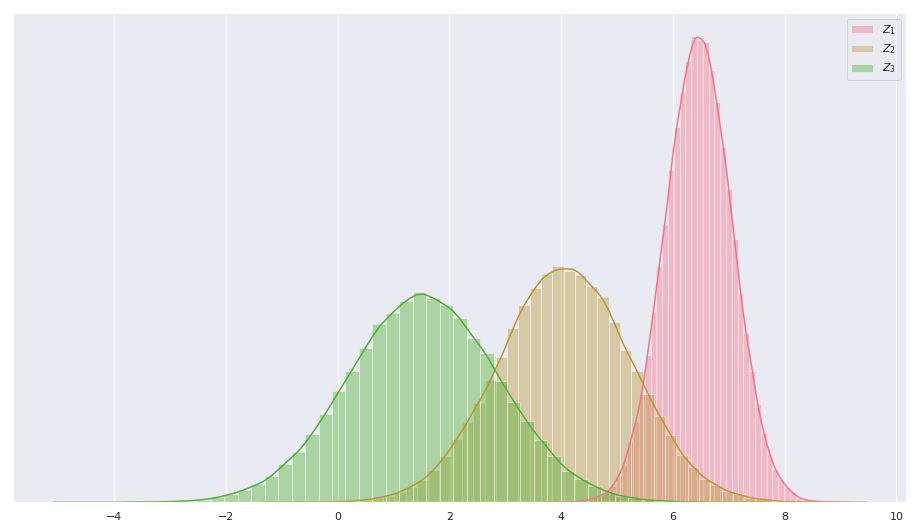
\includegraphics[width=0.8\textwidth]{img/trivariate}
\caption{Example showing density for each univariate distribution given samples from a trivariate distribution $p(s, a, s')$.}
\end{center}
\end{figure}

\subsection{Training procedure}

To setup this experiment, we randomly generate the parameters of a trivariate normal distribution and ensure the covariance matrix is positive semi-definite. The \cvae{} is trained with samples from the trivariate distribution in the following way:

First, we sample $(s, a, s')$ from the trivariate distribution. Then, the probabilistic encoder is used to produce $\qphi \given{z}{s', s, a}$. We then modulate the posterior $z$ with the conditional input $s, a$ and use the decoder to predict the distribution $\ptheta \given{s'}{z, s, a}$. We can view this as analogous to the goal of learning the next state $s'$ conditioned on the current state $s$ and control actions $a$.

\begin{figure}
\centering
\captionsetup{size=footnotesize}
\begin{subfigure}{\linewidth}
  \centering
  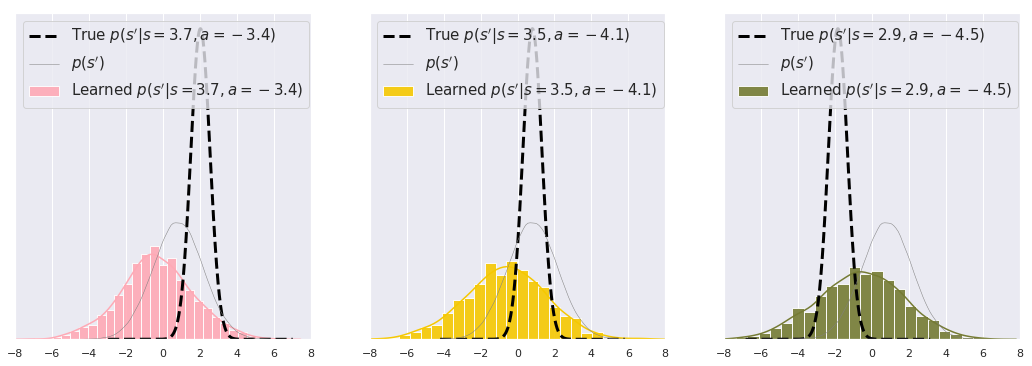
\includegraphics[width=1.0\linewidth]{img/trivariate/trivariate-epoch0}
  \caption{0 gradient steps}
  \label{fig_3_parameters_0}
\end{subfigure}
% \begin{subfigure}{\linewidth}
%   \centering
%   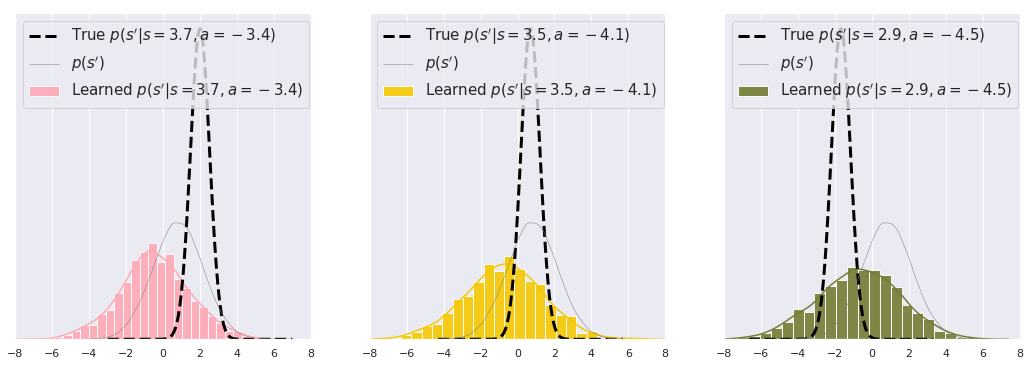
\includegraphics[width=1.0\linewidth]{img/trivariate/trivariate-epoch100}
%   \caption{100 gradient steps}
%   \label{fig_3_parameters_0}
% \end{subfigure}
\begin{subfigure}{\textwidth}
  \centering
  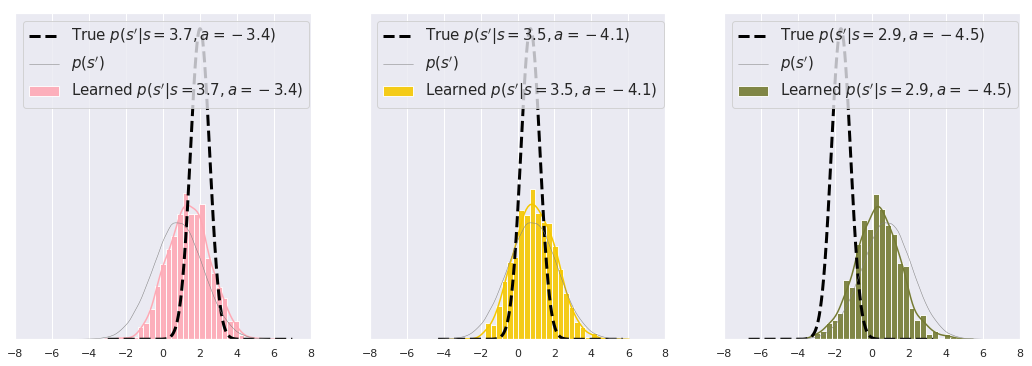
\includegraphics[width=1.0\linewidth]{img/trivariate/trivariate-epoch200}
  \caption{200 gradient steps}
\end{subfigure}
\begin{subfigure}{\textwidth}
  \centering
  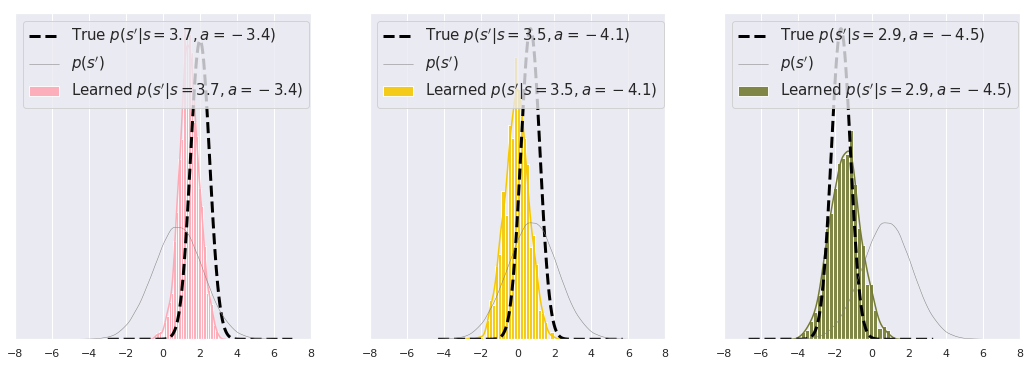
\includegraphics[width=1.0\linewidth]{img/trivariate/trivariate-epoch500.png}
  \caption{500 gradient steps}
\end{subfigure}
\begin{subfigure}{\textwidth}
  \centering
  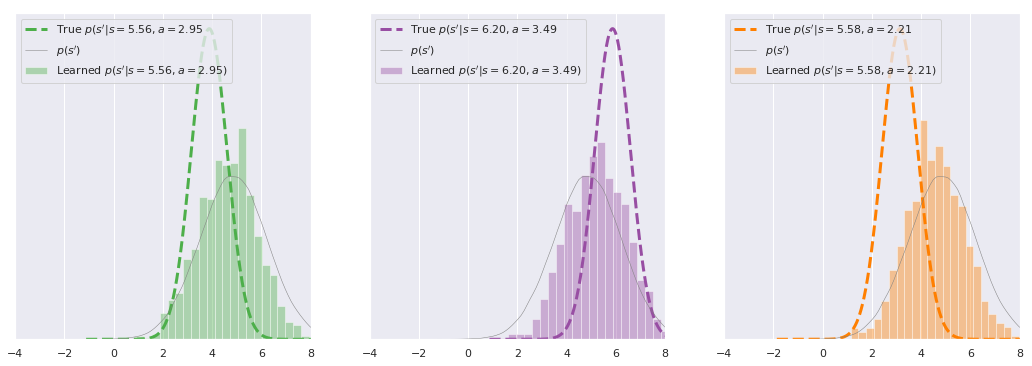
\includegraphics[width=1.0\linewidth]{img/trivariate/trivariate-epoch2000}
  \caption{2000 gradient steps}
\end{subfigure}

\caption[]{Three different density estimations during training for \ensuremath{p \given*{s'}{a,s}} where $a$ and $s$ have been randomly sampled from a known trivariate distribution in each plot and drawn as vertical lines. The expected density $p \given{s'}{s, a} \sim \N (\mu_{\given{s'}{s,a}}, \Sigma_{\given{s'}{s,a}})$ is computed and its outline plotted in thick dashed lines using equations \ref{eq_cond_mean} and \ref{eq_cond_var}.}
\label{fig:trivariate_density}
\end{figure}

As illustrated by Figure \ref{fig:trivariate_density}, the \cvae{} initially learns the distribution $p(s')$ but ultimately converges towards the conditional distribution $p \given{s'}{s, a} \sim \N (\mu_{\given{s'}{s,a}}, \Sigma_{\given{s'}{s,a}})$ after training on enough samples. %That is, the \cvae{} begins learning by ignoring the condition $s, a$, and instead memorizes the distribution $p(s')$, but after seeing enough samples it eventually learns to consider the condition and accurately predicts the conditional distribution $p \given{s'}{s, a}$.

\iffalse
\begin{figure}
\begin{center}
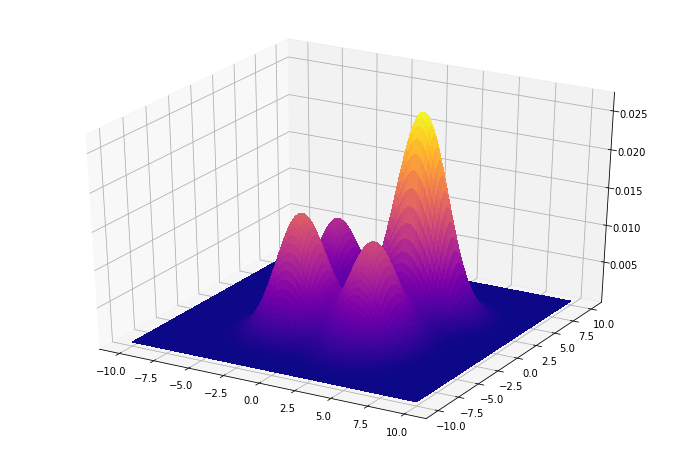
\includegraphics[width=8cm]{img/multimodal_bivariate_3d.png}
\caption{A multimodal mixture of bivariate Gaussians.}
\label{fig_multimodal_bivariate_3d}
\end{center}
\end{figure}
While this indicates that the \cvae{} can learn a conditional distribution, this does not demonstrate that the \cvae{} is capable of learning a multimodal distribution. So as another experiment, we model a bivariate mixture distribution seen in figure \ref{fig_multimodal_bivariate_3d}.

Interestingly, experiments show that increasing the size of the latent space results in a biased distribution that has one mode, rather than being multimodal. Furthermore, even without a mixture model, the \cvae{} can represent multimodal distributions. Results can be seen in figure \ref{fig_multimodal_bivariate}.

\begin{figure}
\begin{center}
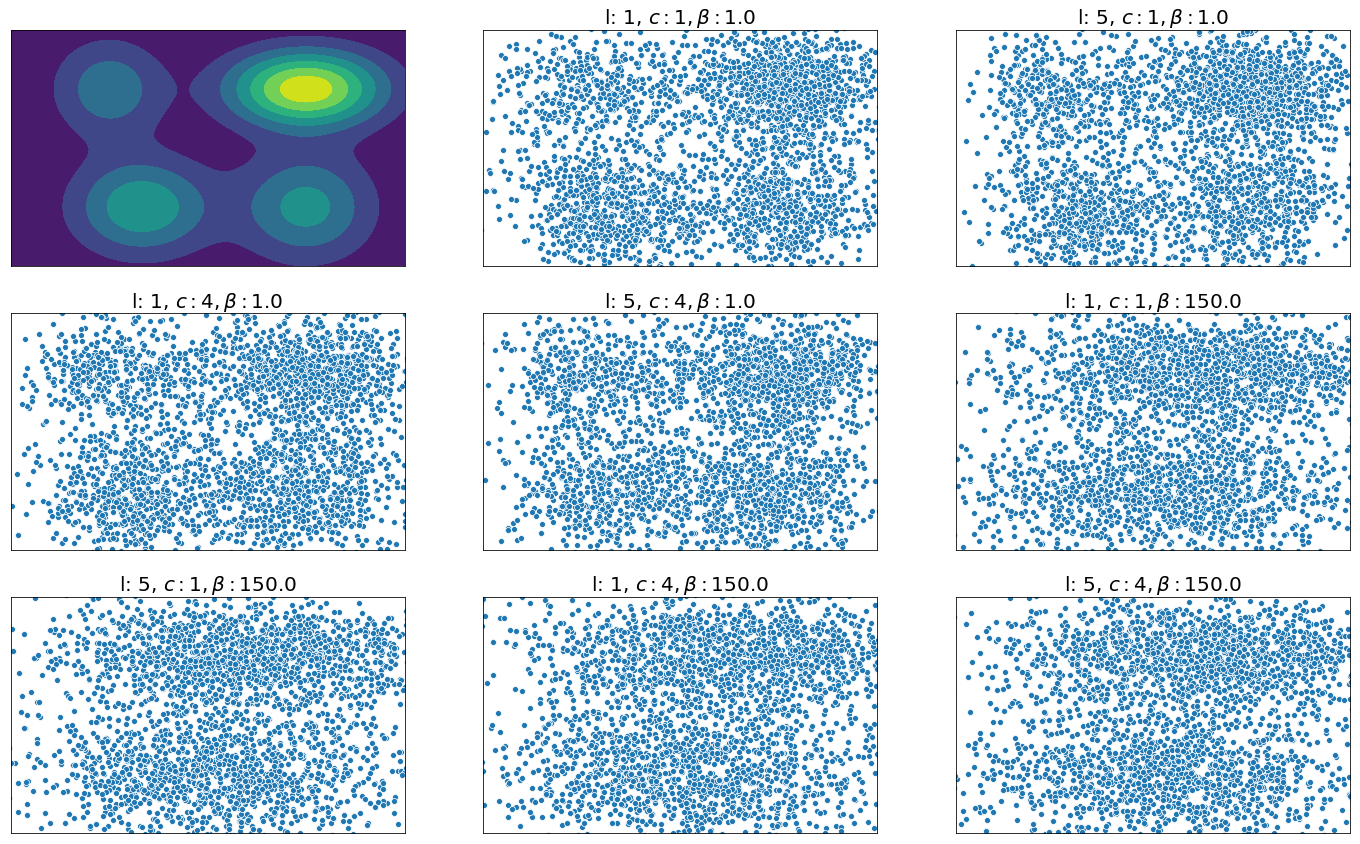
\includegraphics[width=0.8\linewidth]{img/multimodal_bivariate}
\caption{The top left image shows the contour plot of the multimodal mixture distribution. The remaining plots show samples from the decoder using different latent sizes, number of components and changing $\beta$ parameter.}
\label{fig_multimodal_bivariate}
\end{center}
\end{figure}

\fi

\section{The MuJoCo simulator and scenarios}

MuJoCo \parencite{todorov2012mujoco}, short for Multi-Joint dynamics with Contact, is a physics engine, suited in particular for simulating complex dynamic systems in contact-rich scenarios. Performance on robotics-like scenarios simulated by MuJoCo is now frequently reported when analyzing performance of RL algorithms~\parencite{duan2016benchmarking, popov2017data}.

For these experiments, we construct scenarios in MuJoCo and select parameters $\vec{\psi}$ that we wish to learn to reduce the reality gap. %We then observe the scenarios with a distribution over these parameters $\vec{\psi}$. 

In this context, \textit{real} data refers to trajectories generated via the simulator with a known configuration of the parameters with slight Gaussian noise. This noise is introduced during simulation and not added to observations. While this does not guarantee that \dettostoc{} works on actual real-world data, there are other benefits to conducting the experiments this way. One positive bonus with synthesizing \emph{real} data is that we can generate a variety of different physics dynamics to represent different versions of reality and make sure that the algorithm can find the correct set of parameters that best represent that particular system. Moreover, a plethora of test data can be generated to verify the quality of the results.

\subsection{Parameters and their meanings}
In the following experiments when we refer to friction we mean isotropic tangential friction between two geoms in MuJoCo. In MuJoCo, wind is a vector that is subtracted from the 3D translational velocity of each body, and the result is used to compute viscous, lift and drag forces acting on the body. In the Windy Slope scenario, wind is only used along one axis, perpendicular to the inclination of the slope and thus causes the box to move sideways. For more information about how MuJoCo computes friction, contact detection and other forces, please see the Computation part at: \url{mujoco.org/book/computation.html}.

\section{Windy Slope scenario}
\label{windyslope}

\begin{figure}
\begin{subfigure}{\textwidth}
  \centering
  \begin{overpic}[trim=800 100 800 300,clip,width=0.3\textwidth]{img/windyslope/traj/windyslope-real-0}
      \put(2,2) {\color{white}$0s$}
  \end{overpic}
  \begin{overpic}[trim=800 100 800 300,clip,width=0.3\textwidth]{img/windyslope/traj/windyslope-real-50}
      \put(2,2) {\color{white}$2s$}
  \end{overpic}
  \begin{overpic}[trim=800 100 800 300,clip,width=0.3\textwidth]{img/windyslope/traj/windyslope-real-100}
      \put(2,2) {\color{white}$4s$}
  \end{overpic}
\end{subfigure}

\caption{The Windy Slope scenario, where a box with hidden inner content is placed on a sloping surface exposed to wind. A cylindrical obstacle also placed on the surface. Modelling contact is difficult and and should make predicting the output slightly harder. This figure shows 10 different outcomes given parameters samples from the slightly noisy \textit{real} parameter distributions: $\pfriction \sim \N(0.23, 0.01^2)$, $\pcom \sim \N(0.21, 0.04^2)$ and $\pwind \sim \N(-1.7, 0.05^2)$. The positions and orientations of the box have been superimposed in each image to give a sense of the randomness. The choice of means were picked at random, and the variances were selected to be small yet slightly stochastic to resemble the unpredictability of the real world.}
\label{fig:windyslope_real}
\end{figure}

\begin{figure}
\begin{subfigure}{\linewidth}
    \centering
    \begin{overpic}[trim=800 100 400 300,clip,width=0.4\linewidth]{img/windyslope/traj/windyslope-fake-wind-50}
        \put(2,2) {\color{white}$2s$}
    \end{overpic}
        \begin{overpic}[trim=800 100 400 300,clip,width=0.4\linewidth]{img/windyslope/traj/windyslope-fake-wind-99}
        \put(2,2) {\color{white}$4s$}
    \end{overpic}
    \caption{$\vec{\pwind} \sim \N(-1.25,0.5)$ with $\vec{\pfriction}$ and $\vec{\pcom}$ fixed.}
    \label{fig:traj_wind}
\end{subfigure}
\begin{subfigure}{\linewidth}
    \medskip
    \centering
    \begin{overpic}[trim=800 100 400 300,clip,width=0.4\linewidth]{img/windyslope/traj/windyslope-friction-50}
        \put(2,2) {\color{white}$2s$}
    \end{overpic}
        \begin{overpic}[trim=800 100 400 300,clip,width=0.4\linewidth]{img/windyslope/traj/windyslope-friction-99}
        \put(2,2) {\color{white}$4s$}
    \end{overpic}
    \caption{$\vec{\pfriction} \sim \N(0.25,0.1)$ with $\vec{\pwind}$ and $\vec{\pcom}$ fixed.}
    \label{fig:traj_friction}
\end{subfigure}
%
\begin{subfigure}{\linewidth}
    \medskip
    \centering
    \begin{overpic}[trim=800 100 400 300,clip,width=0.4\linewidth]{img/windyslope/traj/windyslope-fake-brick-i-1}
        \put(2,2) {\color{white}$0s$}
    \end{overpic}
    \begin{overpic}[trim=800 100 400 300,clip,width=0.4\linewidth]{img/windyslope/traj/windyslope-fake-brick-i-50}
        \put(2,2) {\color{white}$2s$}
    \end{overpic}
    \caption{Inner box placed at $\pcom=\{-0.45, 0, 0.45\}$.}% from left to right respectively.}
    \label{fig:traj_inner_box}
\end{subfigure}
%
\begin{subfigure}{\linewidth}
    \medskip
    \centering
    \begin{overpic}[trim=800 100 400 300,clip,width=0.4\linewidth]{img/windyslope/traj/windyslope-fake-all-50}
        \put(2,2) {\color{white}$2s$}
    \end{overpic}
        \begin{overpic}[trim=800 100 400 300,clip,width=0.4\linewidth]{img/windyslope/traj/windyslope-fake-all-100}
        \put(2,2) {\color{white}$4s$}
    \end{overpic}
    \caption{All three parameters sampled from initial estimate for $\vec{\psi}.$}
    \label{fig:traj_fake_all}
\end{subfigure}
\caption{Similar to Figure \ref{fig:windyslope_real}, this figure shows snapshots of the environment with parameters sampled from the initial simulation parameters $\vpsi$. To illustrate how each parameter affects the dynamics of the environment, (\subref{fig:traj_wind}) shows the impact of varying wind while keeping the other variables fixed. Similarly, (\subref{fig:traj_friction}) shows varying friction affects with the other variables kept fixed. (\subref{fig:traj_inner_box}) shows three boxes each with the inner box placed in different locations. In (\subref{fig:traj_fake_all}), all three parameters are sampled from $\vpsi$.}
\label{fig:windyslope}
\end{figure}

A first scenario was constructed using MuJoCo in order to see if the \dettostoc{} algorithm can predict the next state given the current state while only simulating passive dynamics.

In this scenario, which can be seen in Figure \ref{fig:windyslope_real} and Figure \ref{fig:windyslope}, an object is placed on a sloping surface. To make the scenario more challenging and to emulate a situation where a parameter cannot be measured, another object is placed inside the box at an unknown position, thus altering the center of mass of the box. How the box moves on the surface depends on the tangential friction coefficients between the surface and the box, $\pfriction$, its center of mass, $\pcom$, as well as viscous, lift and drag forces caused by wind, $\pwind$.

The goal is now to predict the next state $\vns$ given current state $\vs$, with no knowledge of the \textit{real} variables for friction and wind. The state is an 18-dimensional vector consisting of the current position, orientation, linear and angular velocity of the object.

Following the \dettostoc{} algorithm outlined in \ref{det2stoc:algorithm}, we define initial distributions in parameter space $\vec{\psi}$ as wide truncated Gaussians. For this experiment, these initial estimates are purposely made uninformative as a proof of principle. In reality however, the estimates can be based on observing the dynamics in the real world and trying to replicate the same behavior in the simulator.

The position and velocity of the object are recorded every 40ms during four seconds, corresponding to 100 timesteps. Each time the environment is reset, new parameters are sampled from $\vpsi$.

%During the first trial, to keep things less complex, we keep two of the variables fixed while strictly varying the third. This ensures that the particular variable can be identified without interference of the other two variables. The results can be seen in Figure \ref{fig_1_parameter}.

We vary all three parameters: \textit{friction, incline, wind}. The results can be seen in Figure \ref{fig_3_parameters_table}, and visual plots showing the latent space encodings converging towards the \emph{real} parameters Figure \ref{fig:windyslope_latent_space}.

%Then, using \textit{real} data, the \cvae{} is trained to output the next state given current state. We restrict the latent space to be equal to the number of variable parameters, in this case three: \textit{friction, impratio} and \textit{wind}.


%In theory, what is likely to happen is that the latent space captures the underlying parameters that would align simulations with the real world.
%To see if \dettostoc{} can generalize to more than one parameter, we simply choose an arbitrary value for another parameter and collect data in simulation on a range of reasonable values.

\begin{figure}
    \centering
    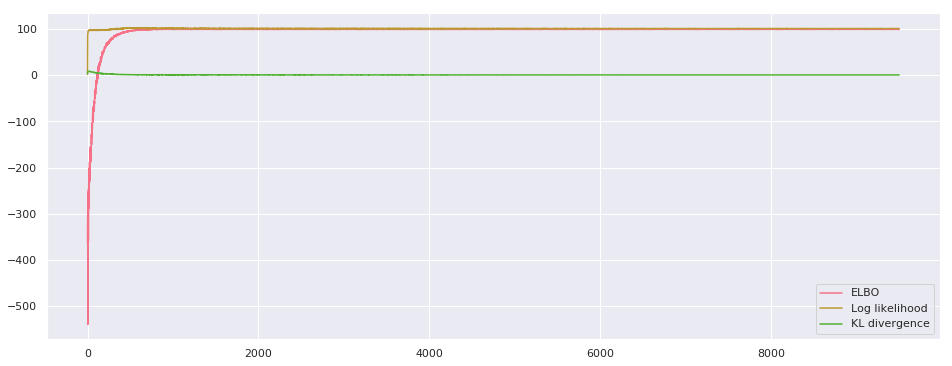
\includegraphics[width=\textwidth]{img/windyslope/windyslope_elbo.png}
    \caption{ELBO plotted of validation set during training of ''real'' data $\vec{\xi}$}
    \label{fig:my_label}
    \todo[inline]{Will fix this plot.}
\end{figure}

\begin{table}
\ra{1.3}
\centering
\begin{tabular}{lrr}
\toprule
%& \multicolumn{2}{c}{\small\emph{Real}} & \phantom{a} & \multicolumn{2}{c}{\emph{Sim}} \\
%\cmidrule{2-3} \cmidrule{5-6}
Model & \# trajectories (samples) & Log likelihood  \\
\midrule
%\cvae{} (baseline) & 5 (500) & 22.09 \\
% 67.285225  65.5517 65.54707 64.27985 68.14507
\cvae{} (baseline) & 10 (1000) & 66.16 $\pm$ 0.69\\

% 20: 85.45479
% 92.60568
%\cvae{} (baseline) & 100 (10000) & 37.14 \\
%\cvae{} (baseline) & 500 (50000) & 41.54 \\

\dettostoc{} (1 iter) & 10 (1000) & -38.49 $\pm$ 0.54 \\
\dettostoc{} (2 iter) & 10 (1000) & 44.39 $\pm$  \\
\dettostoc{} (4 iter) & 10 (1000) & 79.36 $\pm$ 0.0056 \\
\bottomrule
\end{tabular}
\caption{Log probability results test set on the windy slope scenario.}
\label{fig:windyslope_logprob}
\end{table}

\begin{figure}

\centering
\captionsetup{size=footnotesize}
\begin{subfigure}{\linewidth}
  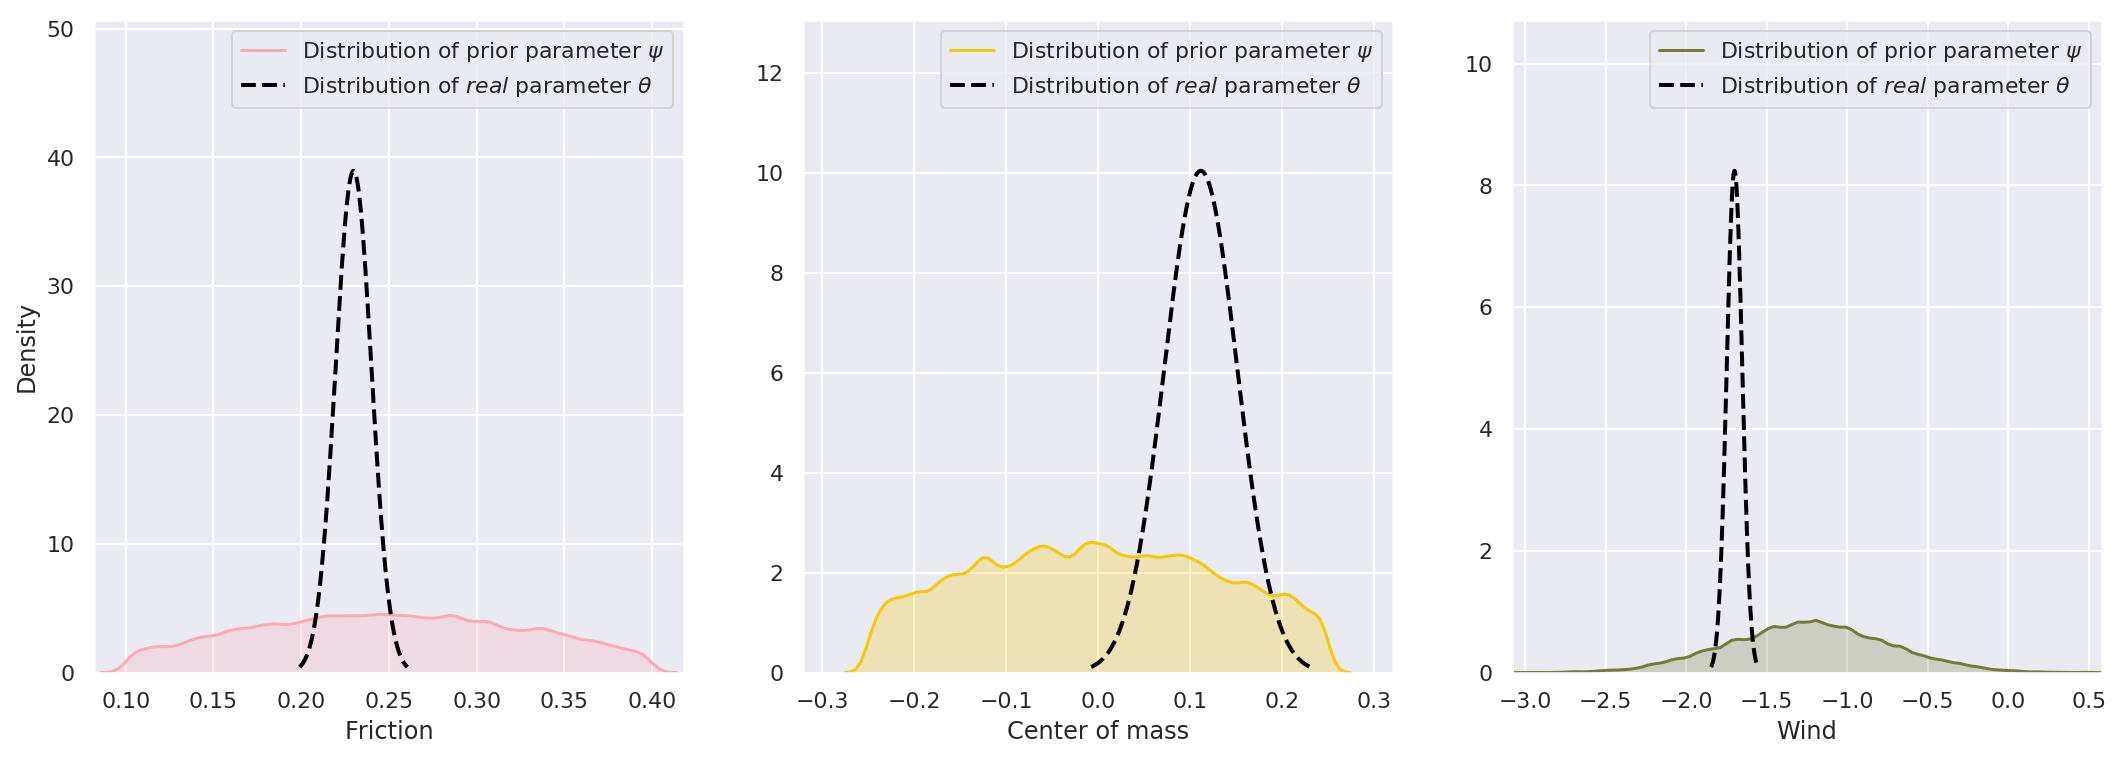
\includegraphics[width=1.0\linewidth]{img/windyslope/latent-representation/new/iter0}
  \caption{Initial estimates of $\psi$}
  \label{fig_3_parameters_0}
\end{subfigure}
\begin{subfigure}{\linewidth}
  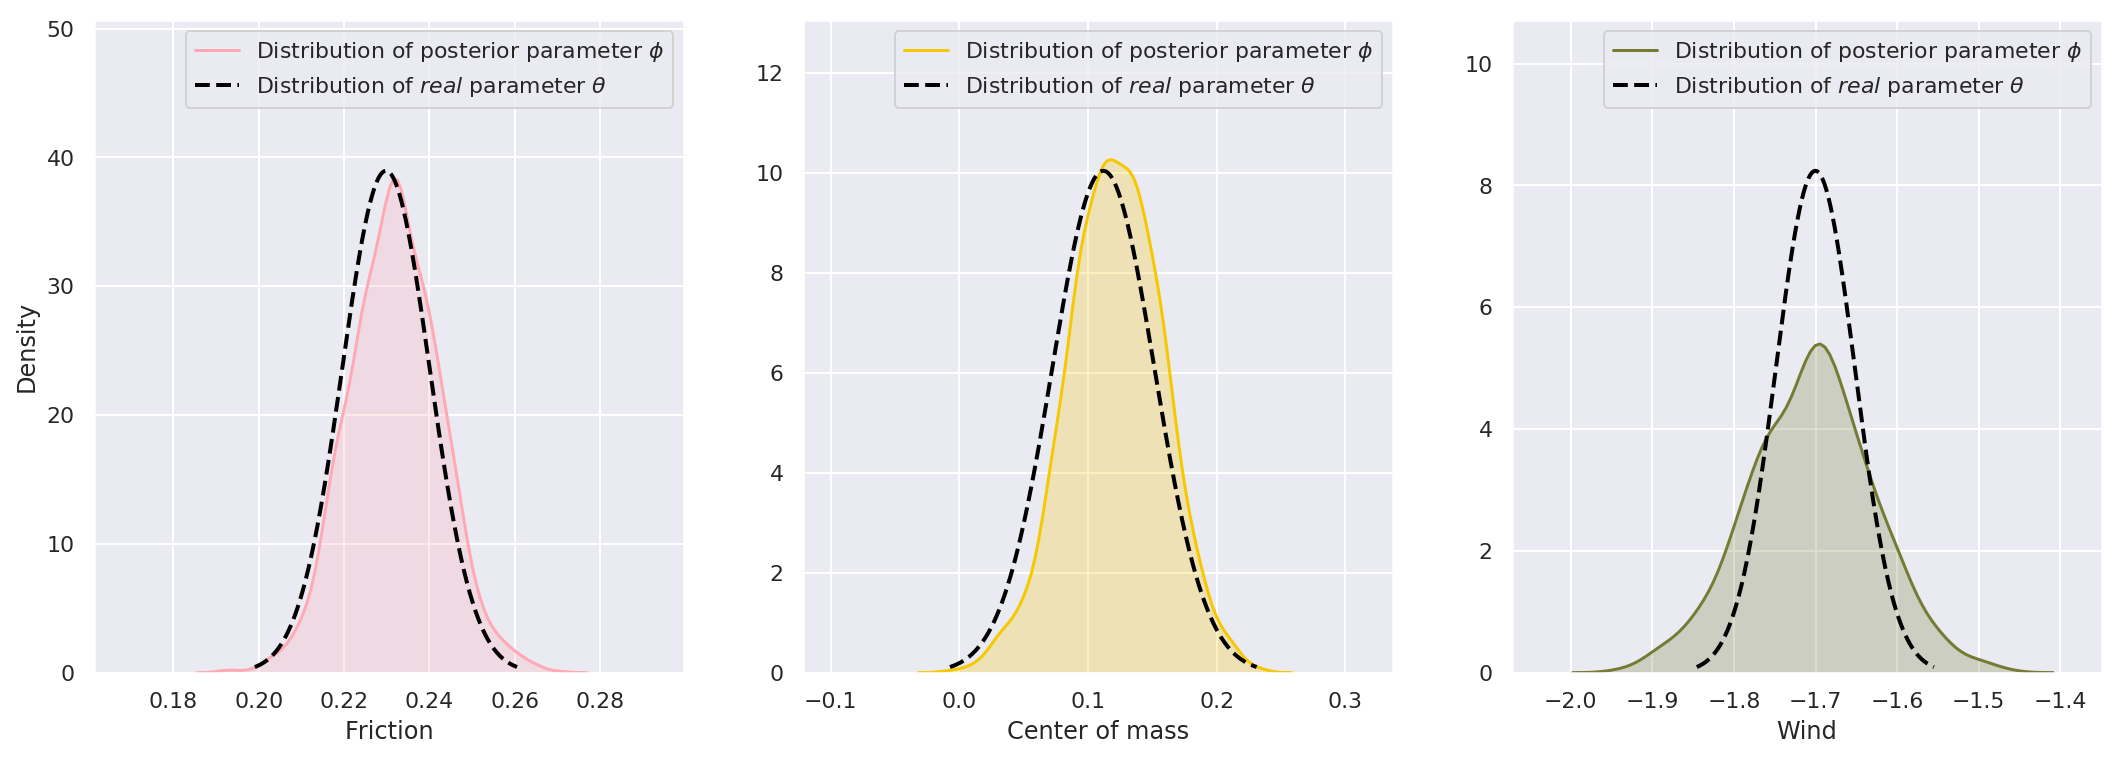
\includegraphics[width=1.0\linewidth]{img/windyslope/latent-representation/new/latent_encoding_iter3}
  \caption{$\psi$ after 3rd iteration of \dettostoc{}}
\end{subfigure}
\caption{Plots show the learned parameters $\vph_{\mu, \sigma}$ of the posterior given \emph{real} samples $\vec{\xi}^{real}$ as normalized histograms after 3 iterations of \dettostoc{}.
From left-to-right, the latent space codings show tangential friction, center of mass and wind. %The prior parameters $\vpsi$ for each iteration of \dettostoc{} are included for clarity in a lighter color, along with the true distribution $\theta_{\mu, \sigma}$ in black dashes.}
The \emph{real} distribution of the parameters $\theta_{\mu, \sigma}$ in drawn with black dashes.}
\label{fig:windyslope_latent_space}

\end{figure}

We compare the results of \dettostoc{} against a \textbf{baseline} \cvae{} with the same number of layers and hidden units. This baseline \cvae{} is trained strictly on \emph{real} data and serves as an indication of the predictive performance without alignment with simulation data.
The log likelihood of the test set gives an indication of the quality of the predictions, but it is not very useful in order to understand how accurate the predictions are. It is obvious that the log likelihood of \dettostoc{} is better than a \cvae{} baseline that has only trained on the \emph{real} data. So to instead better understand how \dettostoc{} performs, we compare it to the true underlying dynamics of the system $p \given{\vns}{\vs}$. To do this, we initialize the physics simulator with a fixed state $\vs$, sample from $\vec{\psi}^{(real)}$ and simulate passive dynamics to generate $\vns$. This will give us a probability distribution over the next state $\vns$ that we can compare to the results $\ptheta \given{\vns}{\vs}$ of the \cvae{}. The results for the position and linear velocity can be seen in \ref{fig:output_distribution_step1_posvel_dettostoc} and \ref{fig:output_distribution_baseline}. The full state observation visualization can be found in appendix \ref{appendix}.

\begin{figure}
\centering
\begin{subfigure}{\textwidth}
    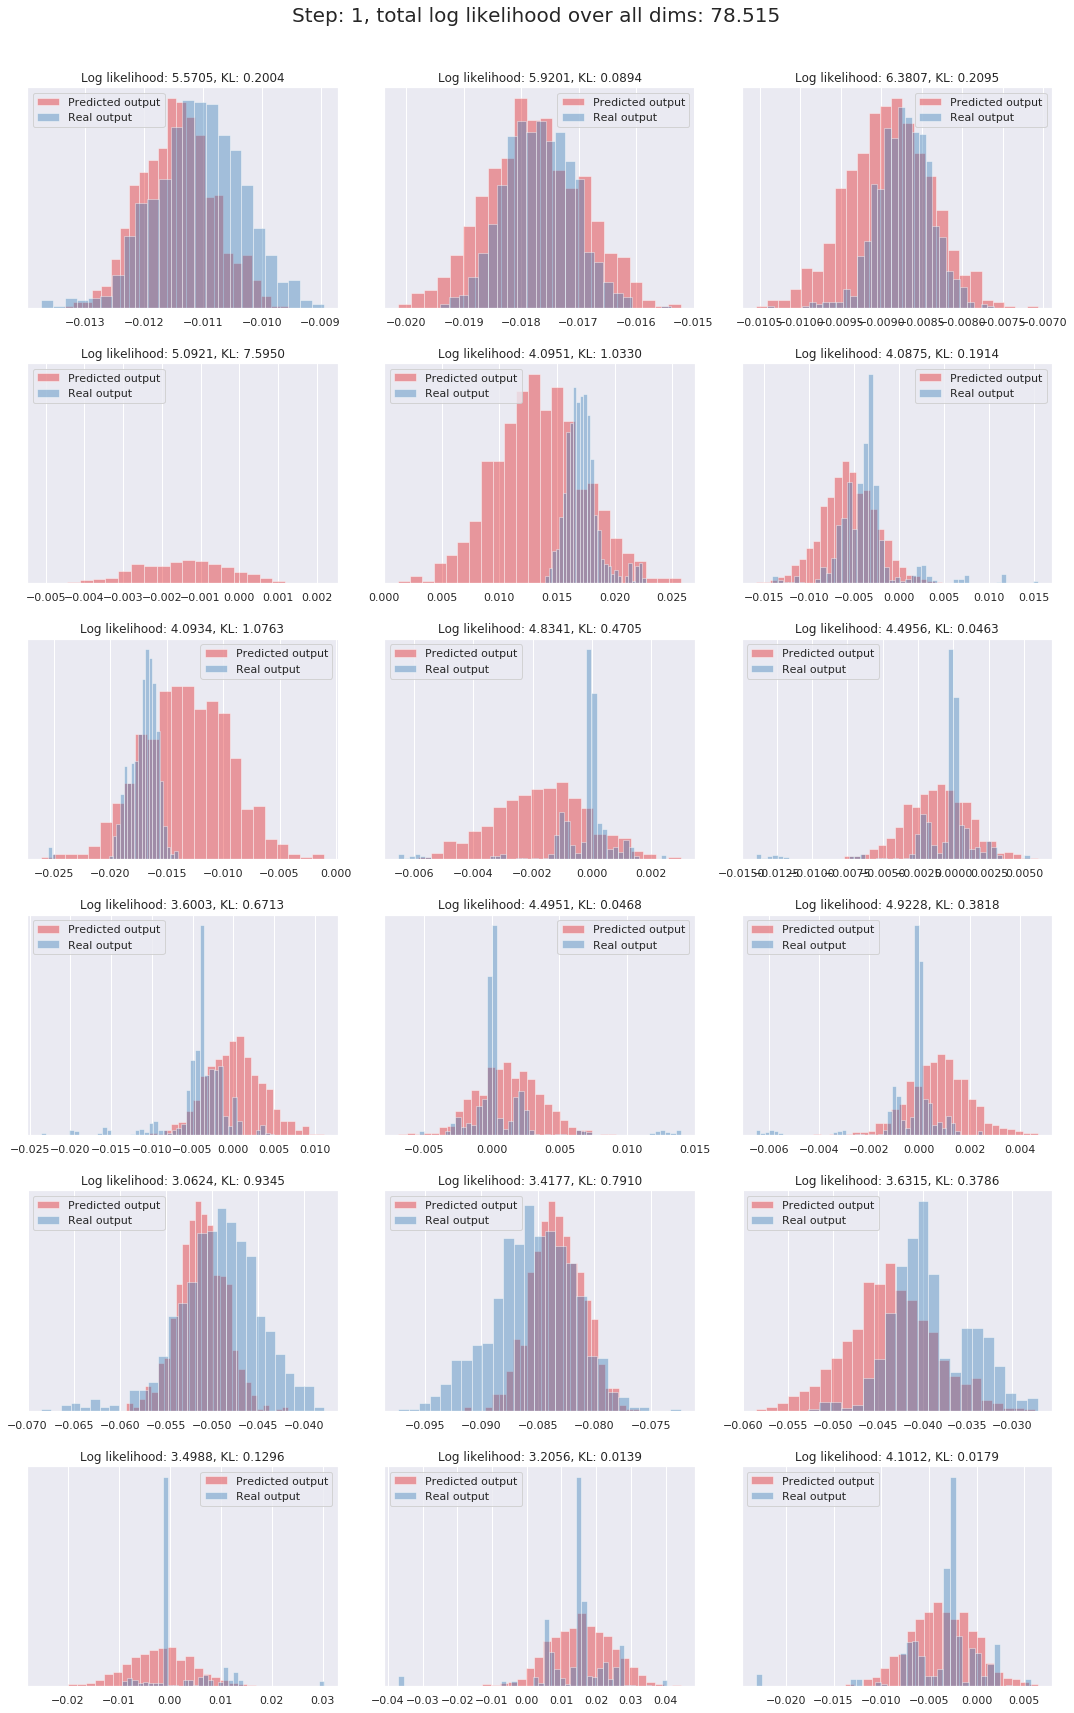
\includegraphics[trim=0 1370 0 50,clip,width=1.0\textwidth]
    {img/windyslope/output/windyslope_output_det2stoc2_dist_10_step1_iter4.png}
    \caption{Output predictions $p_{\vph}\protect\given*{\vns}{\vs}$ for a randomly sampled state at $t=1$ for iteration 4 of \dettostoc{}.}
    \label{fig:output_distribution_step1_posvel_dettostoc}
\end{subfigure}
\begin{subfigure}{\textwidth}
    \centering
    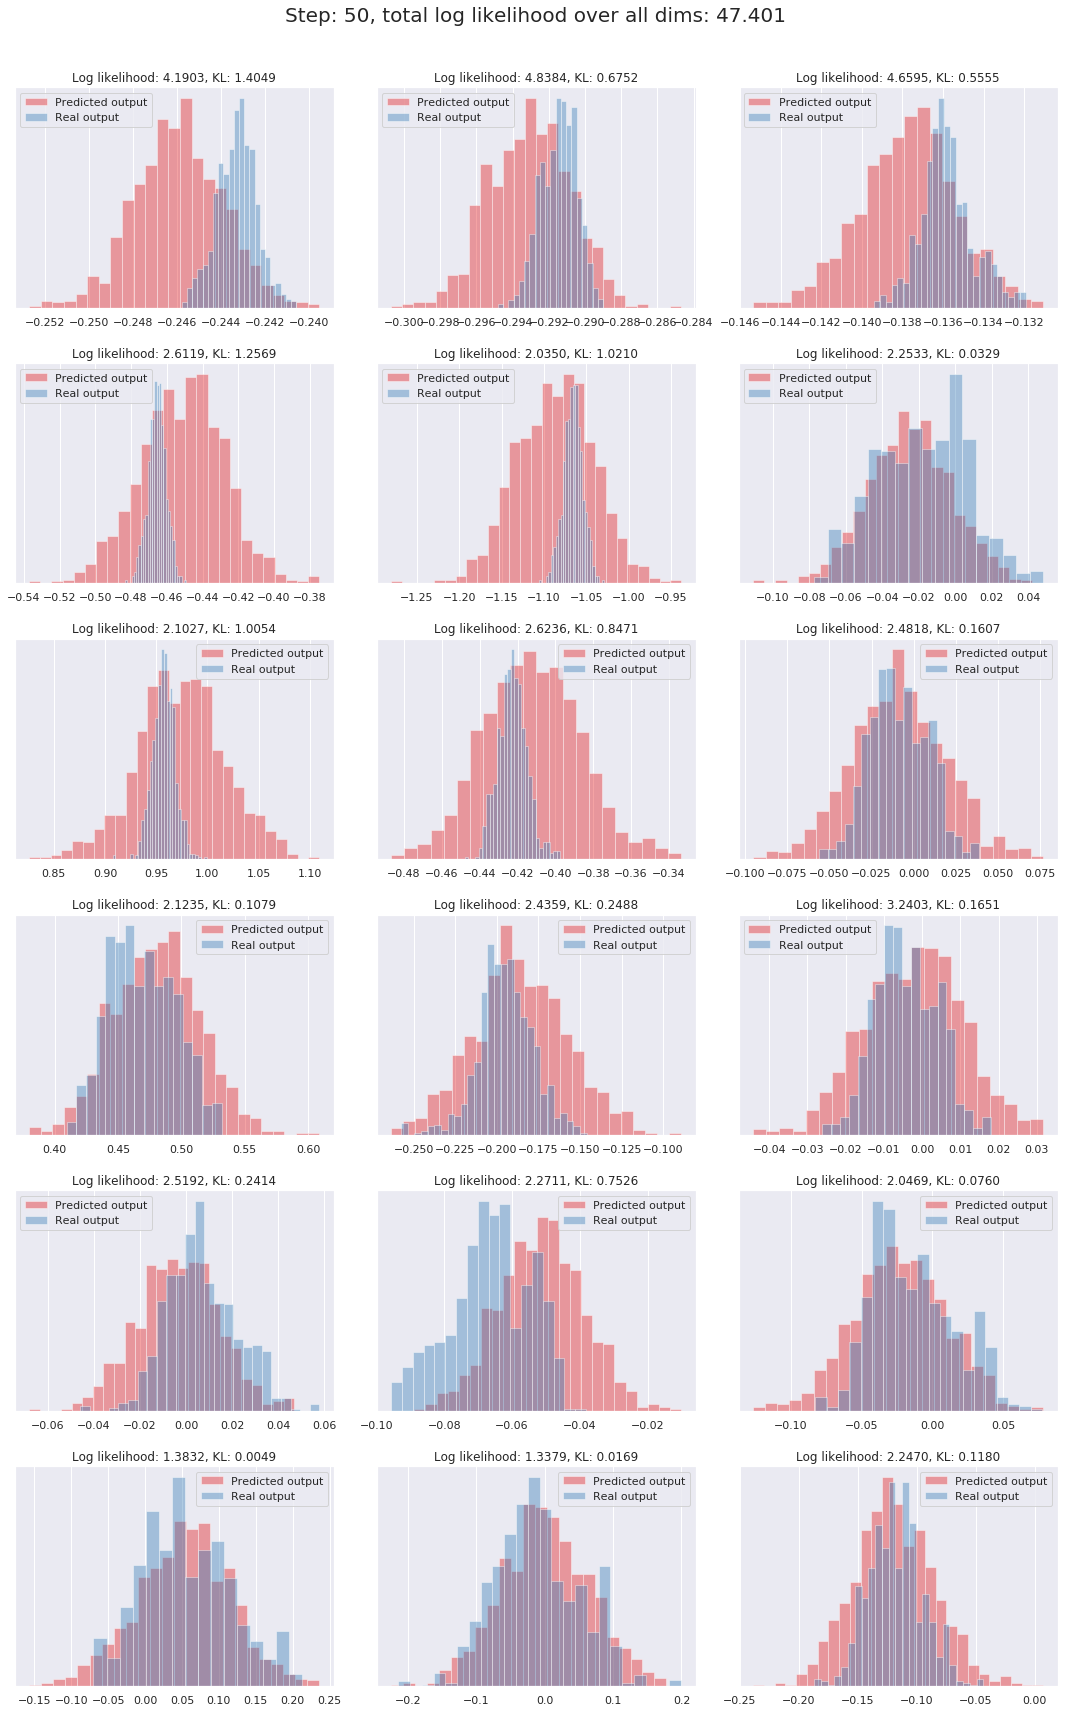
\includegraphics[trim=0 1370 0 50,clip,width=1.0\textwidth]
    {img/windyslope/output/windyslope_output_det2stoc2_dist_10_step50_iter4.png}
    \caption{Output predictions $p_{\vph}\protect\given*{\vns}{\vs}$ for a randomly sampled state at $t=50$ for iteration 4 of \dettostoc{}.}
    \label{fig:output_distribution_step50_posvel_dettostoc}
\end{subfigure}
\begin{subfigure}{\textwidth}
    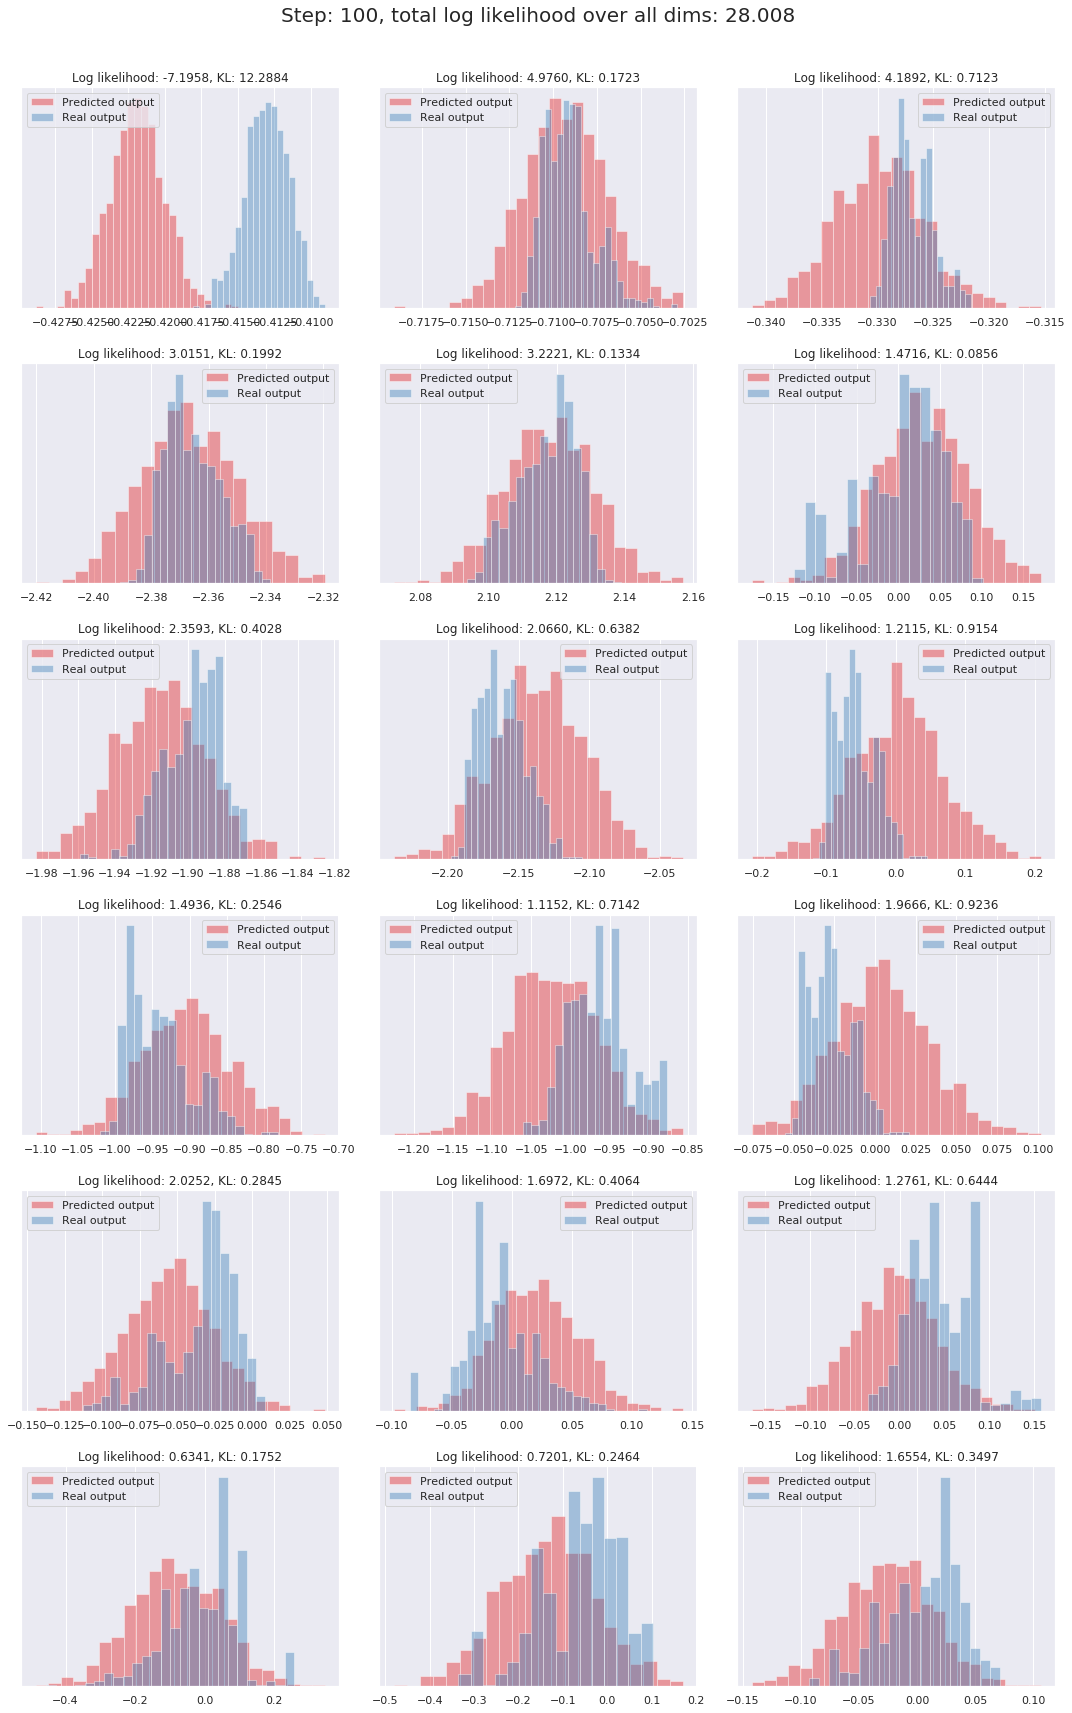
\includegraphics[trim=0 1370 0 50,clip,width=1.0\textwidth]
    {img/windyslope/output/windyslope_output_det2stoc2_dist_10_step100_iter4.png}
    \caption{Output predictions $p_{\vph}\protect\given*{\vns}{\vs}$ for a randomly sampled state at $t=100$ for iteration 4 of \dettostoc{}.}
    \label{fig:output_distribution_step100_posvel_dettostoc}
\end{subfigure}
\begin{subfigure}{\textwidth}
    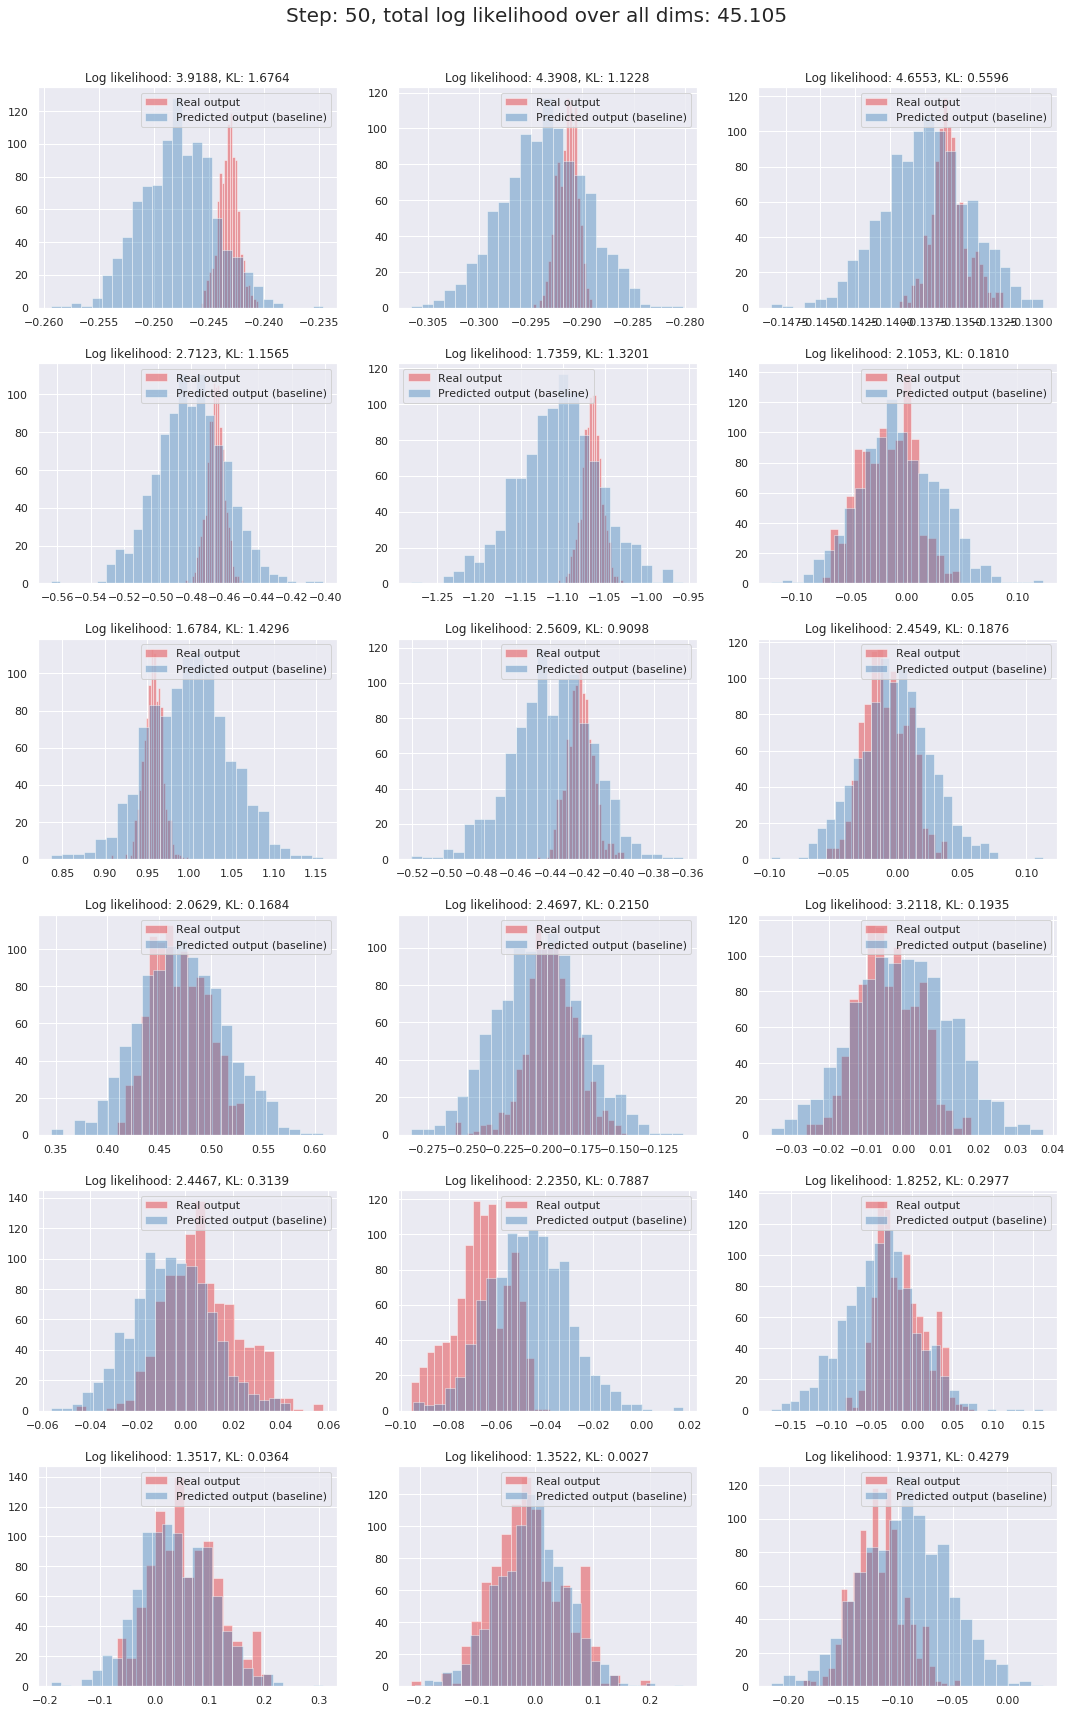
\includegraphics[trim=0 1370 0 0,clip,width=1.0\textwidth]
    {img/windyslope/output/windyslope_output_baseline_dist_10_step50.png}
    \caption{Output predictions $p_{\vph}\protect\given*{\vns}{\vs}$ for a randomly sampled state at $t=50$ for CVAE (baseline).}
    \label{fig:output_distribution_step50_posvel_baseline}
\end{subfigure}
% \caption{Distribution over position outputs (x,y,z) from the simulator and the trained stochastic simulator. The full state outputs is found in Appendix \ref{appendix:a}.}
\todo[inline]{This is old data, will refresh with new.}

\end{figure}

% \begin{figure}
%     \centering
%     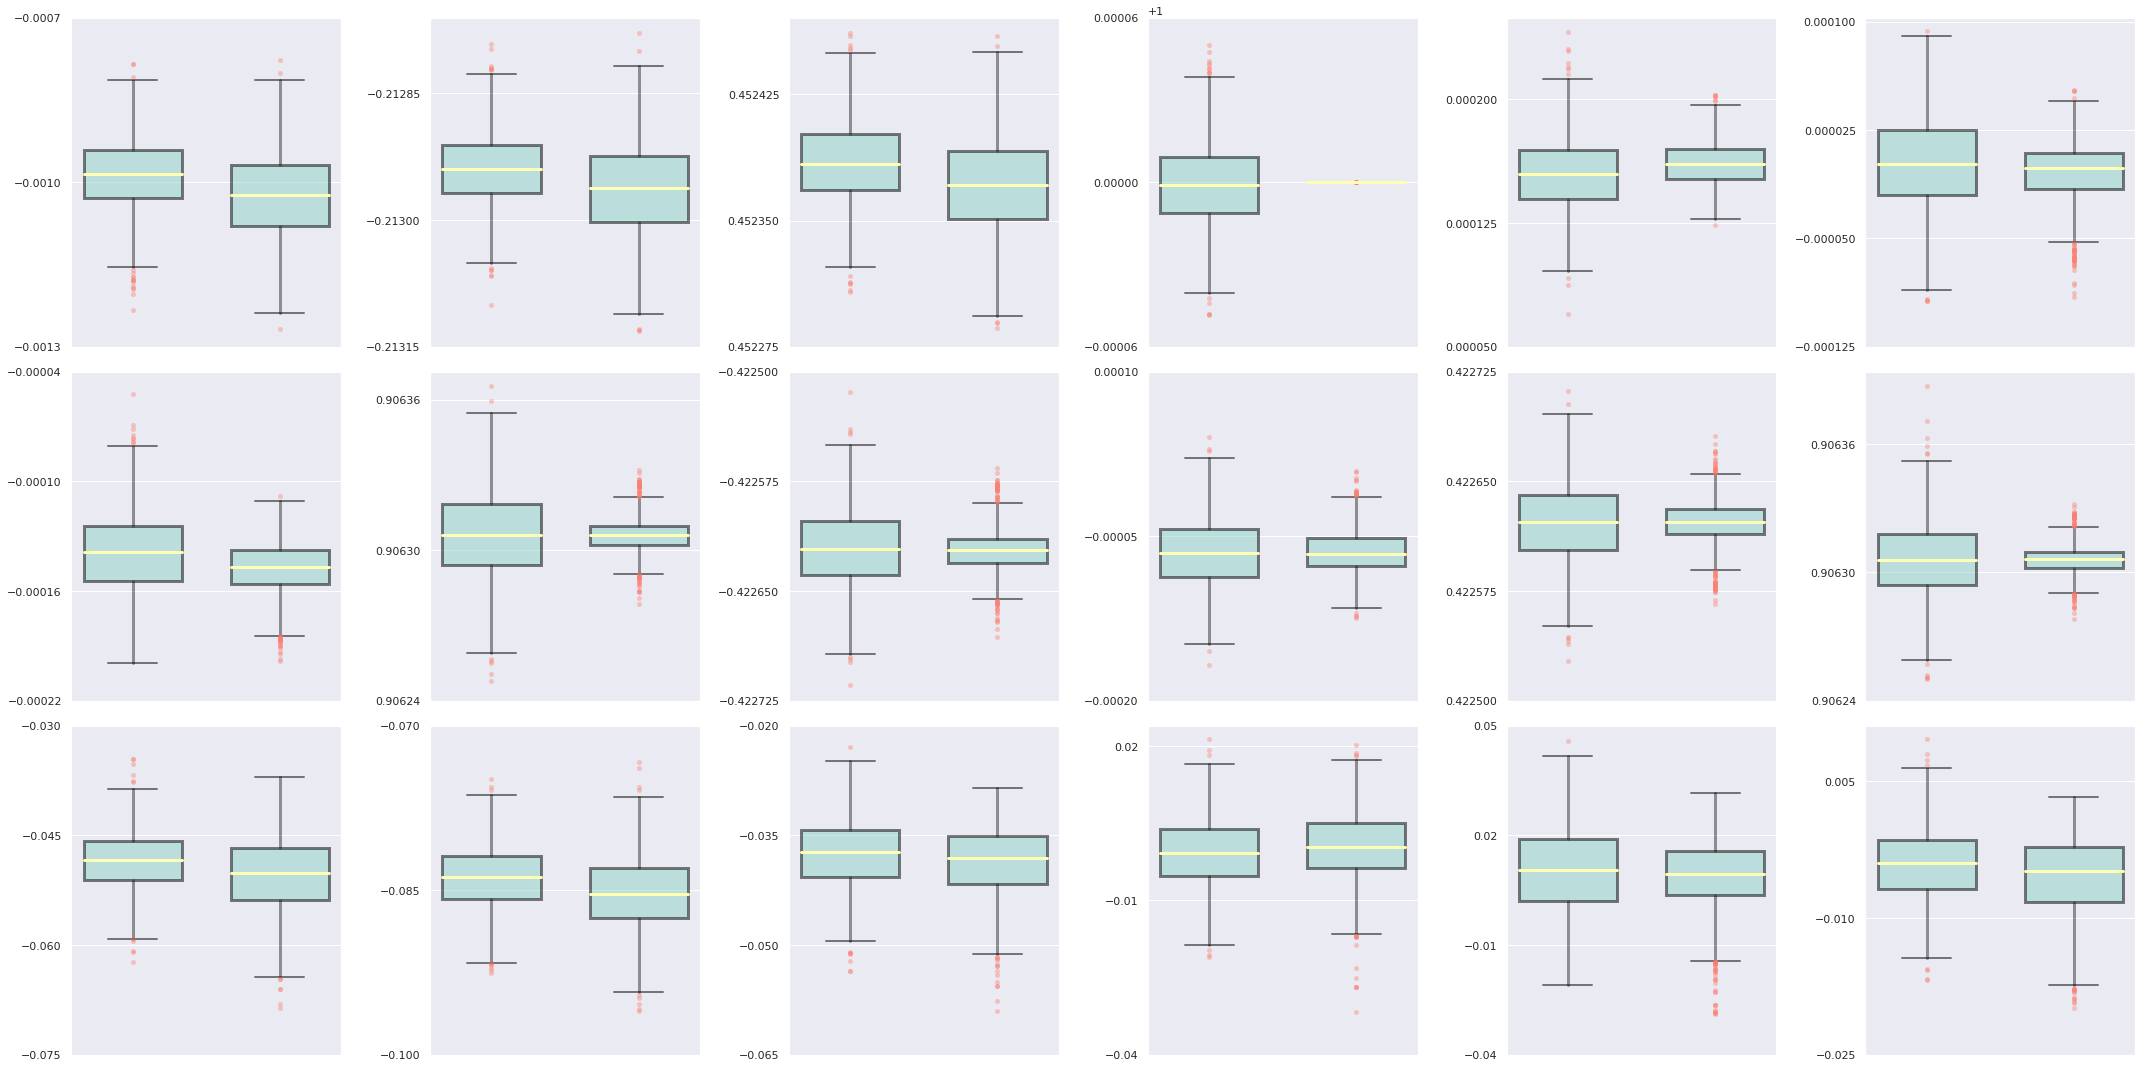
\includegraphics[width=0.8\textwidth]{img/windyslope/output/windyslope_boxplot}
%     \caption{Output predictions for each state as boxplots.}% \todo{Label this properly}}
%     \label{fig:my_label}
% \end{figure}

\subsection{Retrieving parameter predictions using latent space codes}

As an experiment to see if \dettostoc{} can recover the parameters used by \fsimulator{}, we compute the expected mean and standard deviation of the posterior over the \emph{real} training set $\vec{\xi}^{(real)}_{train}$. Since we have included the target $\vns$ in the posterior formulation, and pre-trained the decoder to match \fsimulator{}, samples from $\qphi \given{\vz}{\vs, \vns}$ should approach the true parameters $\vth$. The results can be seen in Table \ref{fig_3_parameters_table} and visually in Figure \ref{fig:windyslope_latent_space}.
%$\E_{\given{\vz}{\vs, \vns}}$

\begin{table}
\ra{1.3}
\centering
\begin{tabular}{lrcrrcrr}
\toprule
%& \multicolumn{2}{c}{\small\emph{Real}} & \phantom{a} & \multicolumn{2}{c}{\emph{Sim}} \\
%\cmidrule{2-3} \cmidrule{5-6}
& $\psi^{(initial)}$ && $\theta_\mu^{(true)}$ & $\phi_\mu^{(learned)}$ && $\theta_\sigma^{(true)}$ & $\phi_\sigma^{(learned)}$ \\
\midrule
$\pfriction$ & $\mathcal{U}$(0.1, 0.4) && 0.23 & 0.2329 && 0.01 & 0.0078 \\
$\pcom$ & $\mathcal{U}$(-0.45, 0.45) && 0.21 & 0.3746 && 0.004 & 0.0188 \\
$\pwind$ & $\mathcal{U}$(-0.5, 3.0) && -1.7 & -1.6949 && 0.05 & 0.0495 \\
\bottomrule
\end{tabular}
\caption{Latent representations of parameters $\psi$ in the windy slope scenario after running two iterations of \dettostoc{} starting from uninformed priors for the parameters $\vec{\psi}$. $\theta_\mu$ and $\theta_\sigma$ correspond to the mean and standard deviation of the \emph{real} parameters of the distribution, and $\phi_\mu$ and $\phi_\sigma$ correspond to the mean and standard deviation of samples from the posterior over the collected \emph{real} trajectories $\vec{\xi}^{real}$.}
\label{fig_3_parameters_table}
\end{table}


\begin{figure}
\centering
\captionsetup{size=footnotesize}
\begin{subfigure}{\linewidth}
  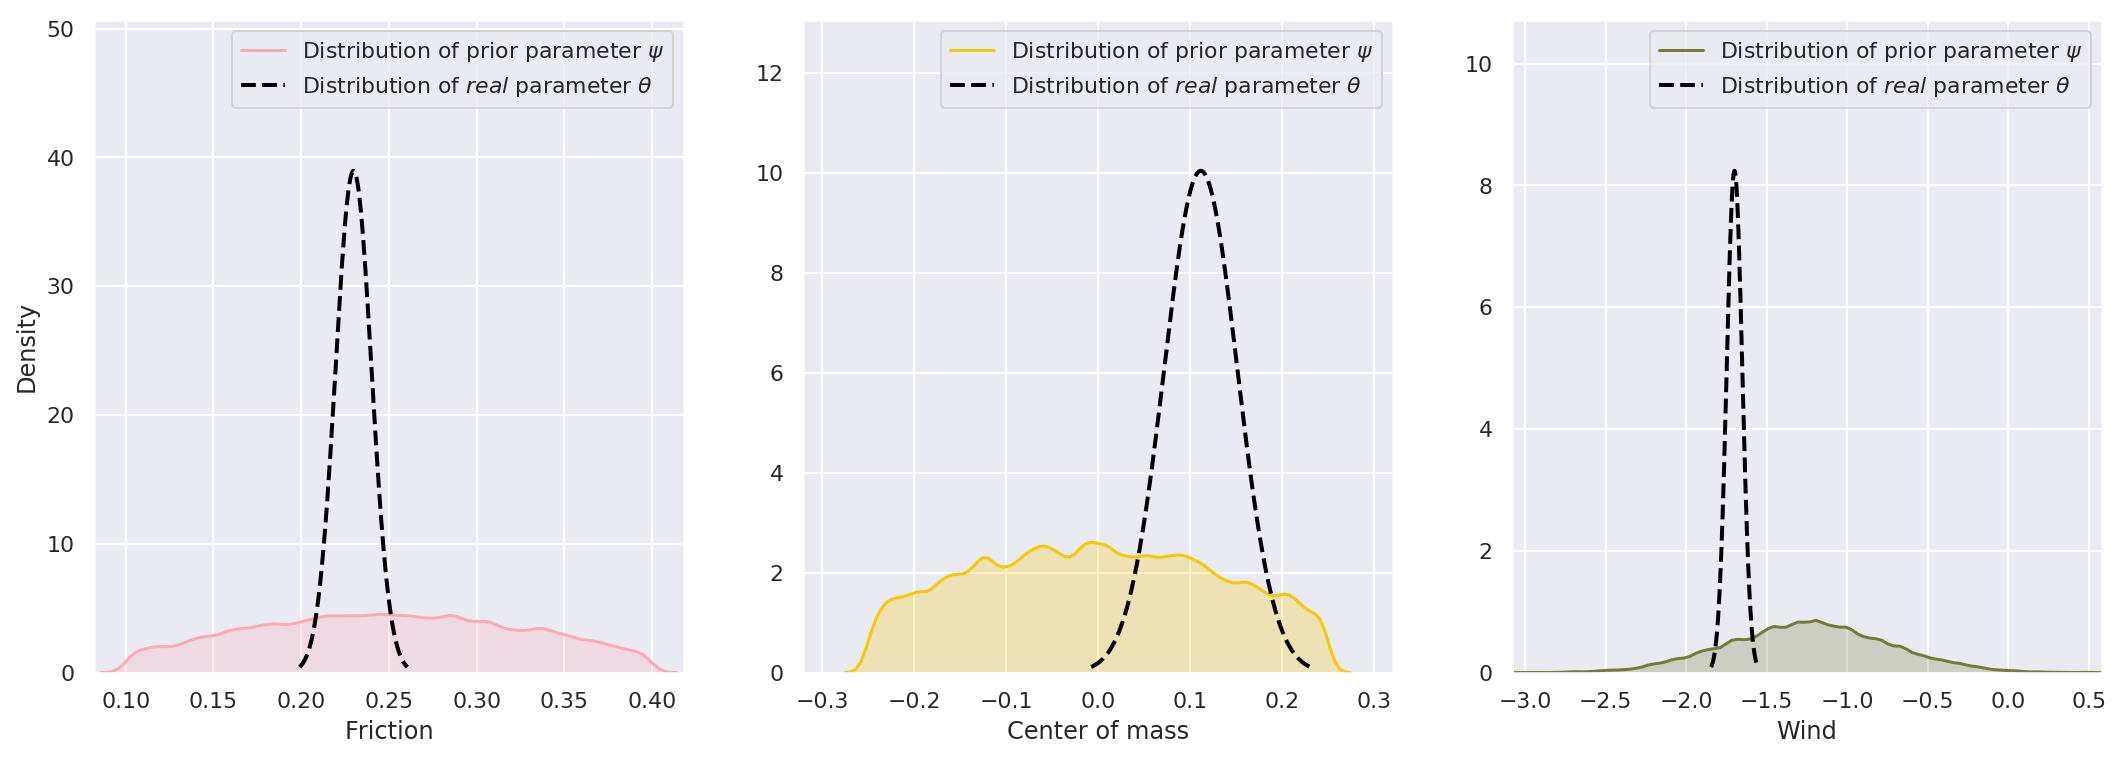
\includegraphics[width=1.0\linewidth]{img/windyslope/latent-representation/new/iter0}
  \caption{Initial estimates of $\psi$}
  \label{fig_3_parameters_0}
\end{subfigure}
\begin{subfigure}{\textwidth}
  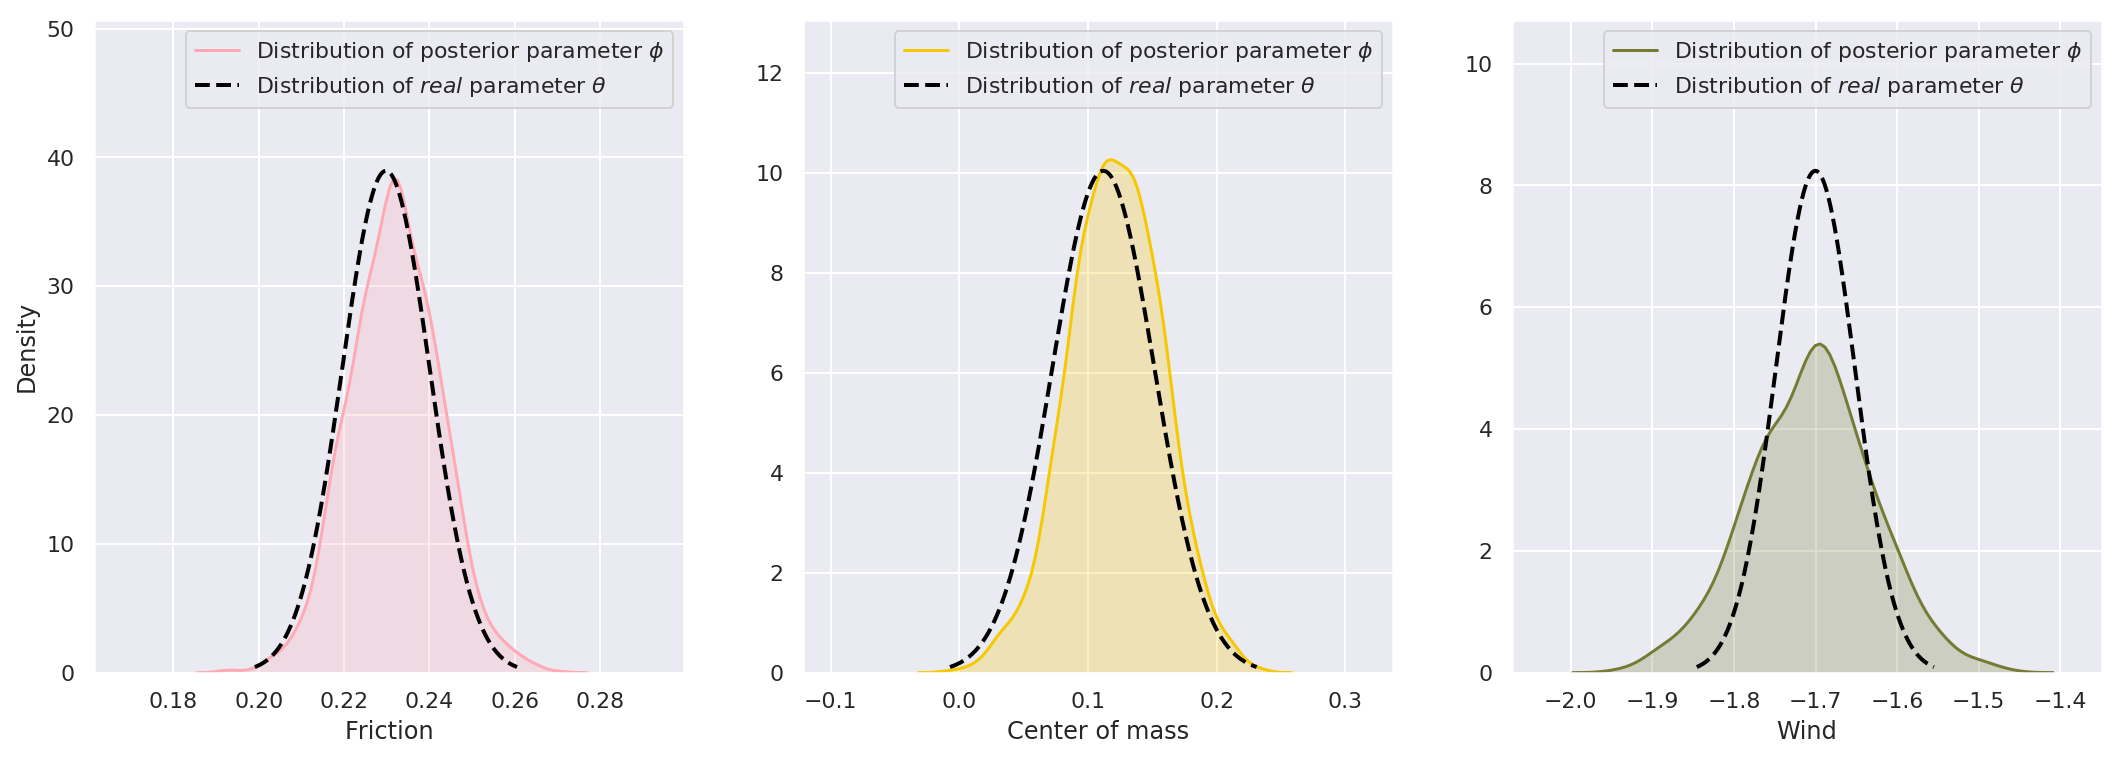
\includegraphics[width=1.0\linewidth]{img/windyslope/latent-representation/new/latent_encoding_iter3}
  \caption{3rd iteration of \dettostoc{}}
\end{subfigure}
\caption{Plots show the learned parameters $\vph_{\mu, \sigma}$ of the posterior given \emph{real} samples $\vec{\xi}^{real}$ as normalized histograms after 3 iterations of \dettostoc{}.
From left-to-right, the latent space codings show tangential friction, center of mass and wind. %The prior parameters $\vpsi$ for each iteration of \dettostoc{} are included for clarity in a lighter color, along with the true distribution $\theta_{\mu, \sigma}$ in black dashes.}
The \emph{real} distribution of the parameters $\theta_{\mu, \sigma}$ in drawn with black dashes. Plots from previous iterations can be found in Appendix \ref{appendix:a}.}
\label{fig:windyslope_latent_space}
\end{figure}

\subsection{YuMi pushing scenario}

A second scenario was constructed in MuJoCo that introduces control actions affecting the system dynamics. Similar to the Windy Slope scenario, a box with unknown center of mass is placed on a surface with unknown friction. However, inclination and wind have been removed and instead a robot interacts with the environment with the goal of pushing the box close to a target goal.

The robot is an ABB IRB14000 YuMi with 2 arms, each with 7 joints corresponding to 14 degrees of freedom. The joints are actuated by velocity controllers. The real robot and the robot modelled in MuJoCo can be seen in Figure \ref{fig:robots}. 

At the start of each episode, the arms are initialized to a default pose and the initial location of the box is placed randomly within a $0.2m \times 0.2m$ square area. The goal is kept fixed in the center of the table. The true friction and center of mass distributions are listed in table \ref{table:yumi-dist}.

The goal is now to predict the next state $\vns$ given $\vs$ and $\va$. The state consists of the position and velocity of all 14 joints as well as the position, rotation and velocity of the box.

%The reward is a function of the distance: it is 0 outside a 0.14m radius of the goal, and otherwise monotonically increasing until the box is within 0.07m of the goal, which yields a reward of 1.


\begin{figure}%
    \centering
    \begin{subfigure}{0.4\textwidth}
    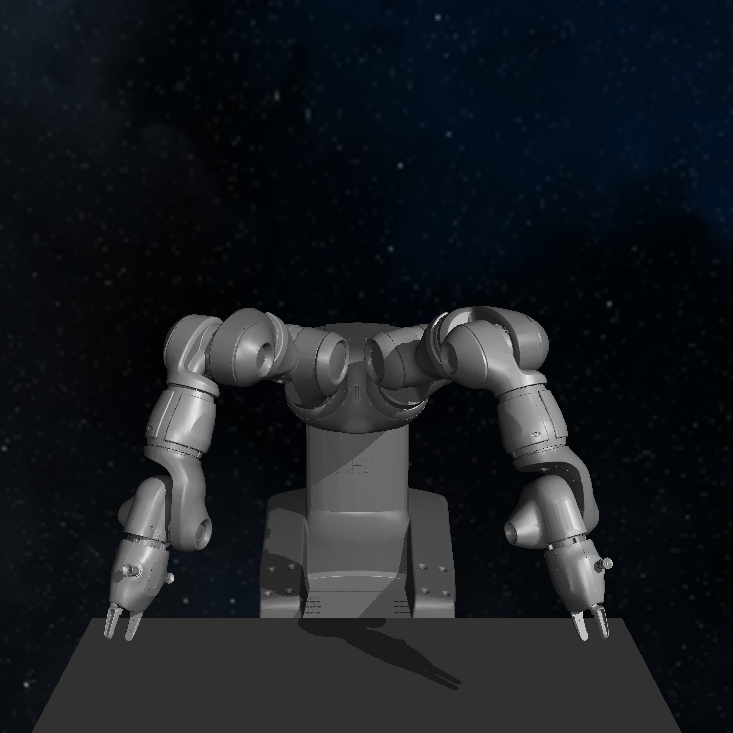
\includegraphics[width=1\textwidth]{img/yumi/yumi-pose-sim}
    \end{subfigure}
    \begin{subfigure}{0.4\textwidth}
    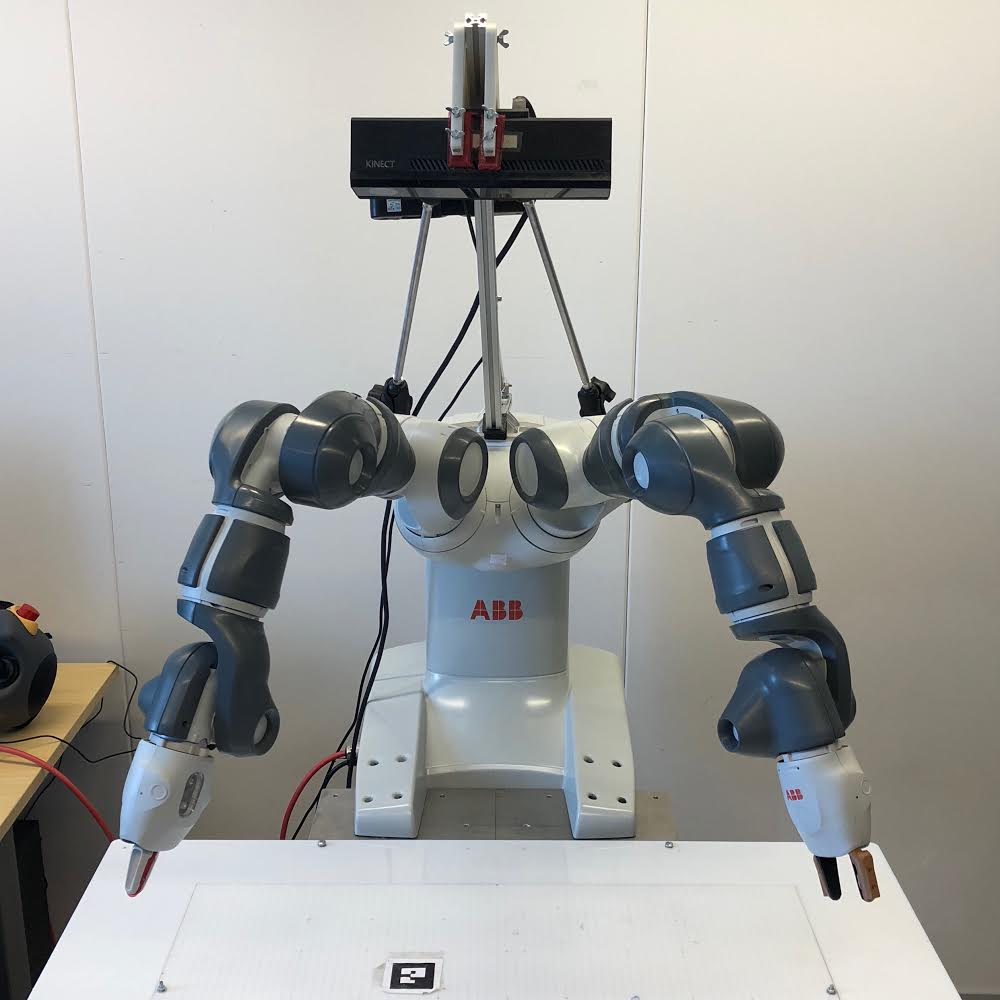
\includegraphics[width=1\textwidth]{img/yumi/yumi-pose-real}
    \end{subfigure}
    \caption{The simulated robot in MuJoCo and the real ABB IRB14000 robot.}
    \label{fig:robots}%
\end{figure}

\begin{table}
\ra{1.3}
\centering
\begin{tabular}{lrrcrr}
\toprule
%& \multicolumn{2}{c}{\small\emph{Real}} & \phantom{a} & \multicolumn{2}{c}{\emph{Sim}} \\
%\cmidrule{2-3} \cmidrule{5-6}
& $\theta_\mu^{(true)}$ & $\phi_\mu^{(learned)}$ && $\theta_\sigma^{(true)}$ & $\phi_\sigma^{(learned)}$ \\
\midrule
$\pfriction$ & $0.28$ & $0.3404$ && $0.01$ & $0.1093$ \\
$\pcom$ & $0.035$ & $ 0.0367$ && $0.005$ & $0.0048$ \\
\bottomrule
\end{tabular}
\caption{Latent representations of parameters $\psi$ in the Windy Slope scenario after running two iterations of \dettostoc{} starting from uninformed priors for the parameters $\vec{\psi}$. $\theta_\mu$ and $\theta_\sigma$ correspond to the mean and standard deviation of the \emph{real} parameters of the distribution, and $\phi_\mu$ and $\phi_\sigma$ correspond to the mean and standard deviation of samples from the posterior over the collected \emph{real} trajectories $\vec{\xi}^{real}$.}
\label{fig_3_parameters_table}
\end{table}


\begin{table}
\ra{1.3}
\centering
\begin{tabular}{lrr}
\toprule
%& \multicolumn{2}{c}{\small\emph{Real}} & \phantom{a} & \multicolumn{2}{c}{\emph{Sim}} \\
%\cmidrule{2-3} \cmidrule{5-6}
Model & \# \emph{Real} trajectories (samples) & Log likelihood over $\trajreal_{test}$ \\
\midrule
\cvae{} (baseline) & 10 (1000) & 306.4443\\
\cvae{} (baseline) & 900 (90000) & 680.5626 \\
\dettostoc{} (1 iter) & 10 (1000) & 673.4169\\
\dettostoc{} (2 iter) & 10 (1000) & 673.9966\\
\dettostoc{} (3 iter) & 10 (1000) & 706.21295\\
\dettostoc{} (4 iter) & 10 (1000) & \textbf{724.1508}\\

\bottomrule
\end{tabular}
\caption{Log likelihood results test set on the YuMi scenario. \dettostoc{} has only seen 1000 \emph{real} samples but still outperforms model that has trained on 9000 samples.}
\label{fig:windyslope_logprob}
\end{table}


\begin{figure}
\centering
\captionsetup{size=footnotesize}
\begin{subfigure}{\textwidth}
  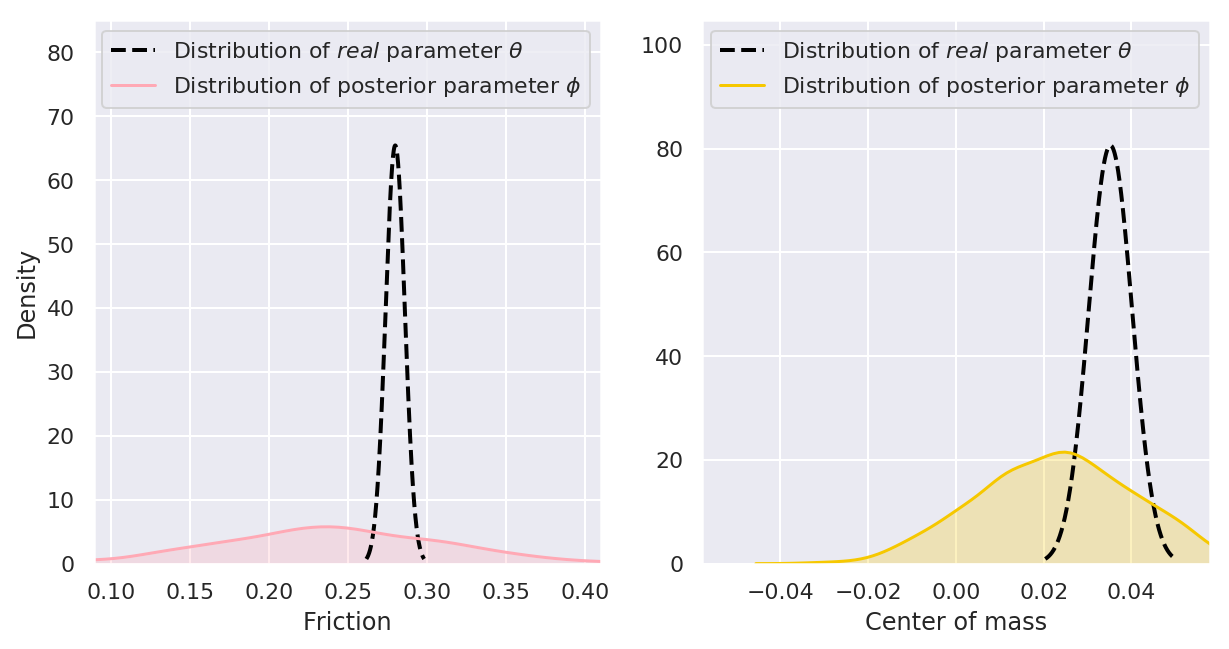
\includegraphics[width=\textwidth]{img/yumi/latent-representation/yumi_latent_encoding_0_iter}%
  \caption{Initial estimates of $\vpsi$ before \dettostoc{}}
\end{subfigure}
\begin{subfigure}{\textwidth}
  \centering
  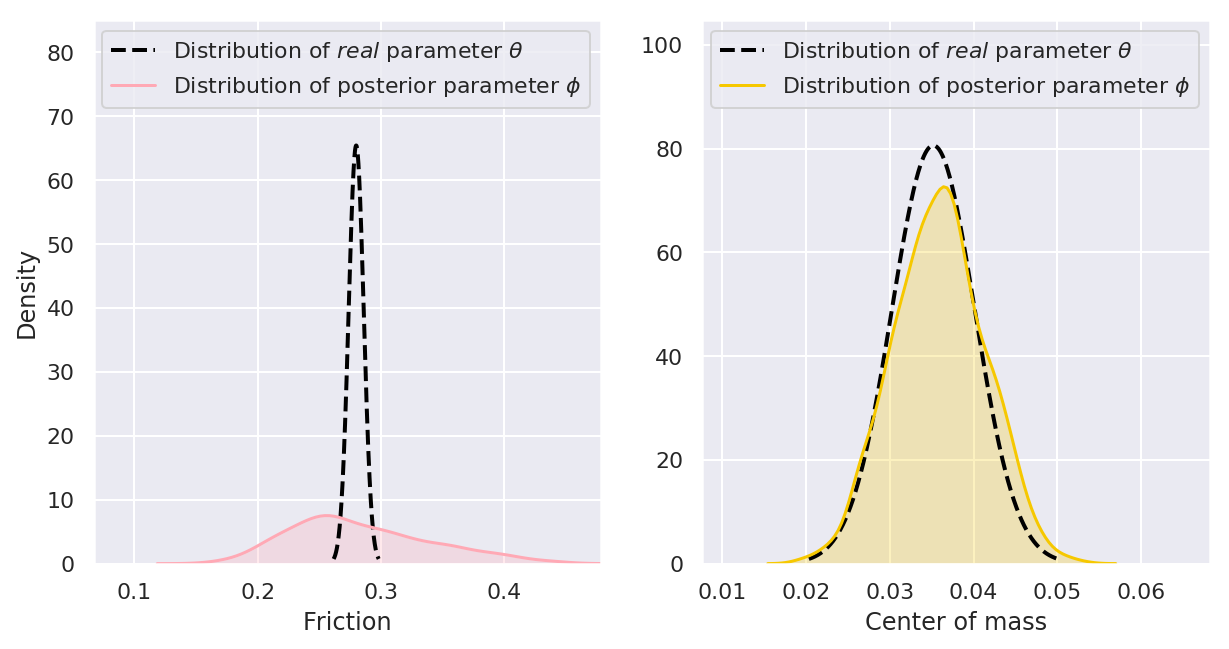
\includegraphics[width=\linewidth]{img/yumi/latent-representation/yumi_latent_encoding_3_iter}
  \caption{3rd iteration of \dettostoc{}}
\end{subfigure}
\caption{Plots show the learned parameters $\vph_{\mu, \sigma}$ of the posterior given \emph{real} samples $\vec{\xi}^{real}$ in the YuMi scenario for four iteration of \dettostoc{}.
The parameters correspond (from left-to-right) to tangential friction $\pfriction$ and center of mass $\pcom$. The true distributions $\vth_{\mu, \sigma}$ are outlined in black dashes. In this scenario, \dettostoc{} struggles to match $\pfriction{}$ with the true distribution $\th_\textsc{friction}$. This is likely due to the fact that the learned policy pushes the box in small increments, and small changes in friction do not cause any noticable difference. The posterior for all iterations can be found in the appendix.}
\label{fig:yumi/latentspace}
\end{figure}